\chapter{Minimalbeispiel 3D-Stereokalibrierung und Szenenrekonstruktion bei Kameras gleicher Auflösung}
\label{sec:minimal} 

Um den Mathematischen Vorgänge der stereoskopischen Szenenrekonstruktion zu veranschaulichen und besser nachvollziehen zu können, wurde ein Minimalszenario erstellt. Mit Hilfe dieses Minimalszenarios, können Theorien besser getestet und bestimmte Situationen simuliert werden. Des Weiteren kann es von Nutzen sein, wenn es darum geht, Fehler in Realbeispielen nachzustellen oder eine Lösung für diese zu finden. Für dieses Minimalszenario wurde ein Objekt, in diesem Falle ein Quader, in ein zuvor definiertes Weltkoordinatensystem $(O,\delta)$ mit $\delta = (d_1,d_2,d_3)$ platziert. Außerdem wurden zwei Kameras $(C,\beta)$ mit $\beta = (b_1,b_2,b_3)$ und $(C',\beta')$ mit $\beta' = (b'_1,b'_2,b'_3)$ definiert und in $(O,\delta)$ platziert. Kamera eins $(C,\beta)$ ist Deckungsgleich mit $(O,\delta)$. Kamera zwei $(C',\beta')$ wurde von $C$ in positive $d_1$-Richtung, verschoben und um einen Winkel $\alpha$ zu $C$ um die eigene $b'_3$-Achse rotiert. Die verwendeten kartesischen Koordinatensysteme sind in diesem Minimalbeispiel alle rechtshändig orientiert. Die äußeren und inneren Kameraparameter wurden für den Aufbau der Szene festgelegt. Dies hat den positiven Effekt, dass somit die späteren Ergebnisse besser validiert werden können. In den Abbildung 4.1 bis 4.3 wird der Aufbau noch einmal genauer veranschaulicht. \\

\begin{figure}[!htb]
	\minipage{0.52\textwidth}
	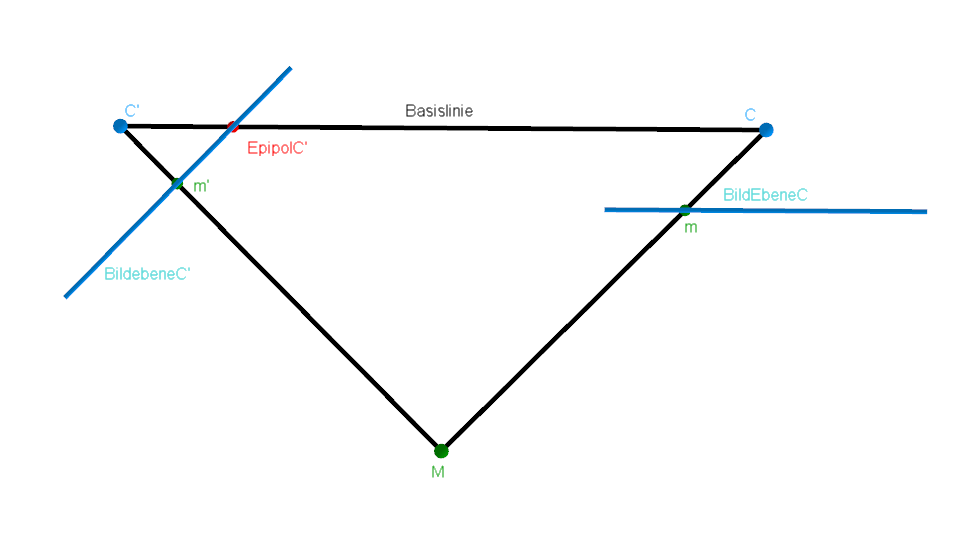
\includegraphics[width=\linewidth]{images/AufbauMinimalbeispiel.png}
	\caption{vereinfachte Top-Down-Ansicht des Szenenaufbaus des Minimalbeipspiels}
	\label{fig:awesome_image1}
	\endminipage\hfill
	\minipage{0.42\textwidth}
	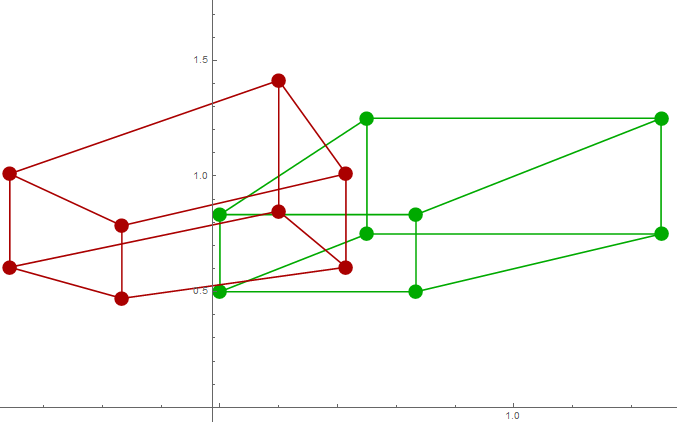
\includegraphics[width=\linewidth]{images/QuadrateMinimalBeispiel.png}
	\caption{In Grün ist die Abbildung auf der Bildebenen $I$ von $C$ und in rot ist die Abbildung auf der Bildebenen $I'$ von $C'$}
	\label{fig:awesome_image2}
	\endminipage\hfill
\end{figure}

\begin{minipage}{\linewidth}
	\centering
	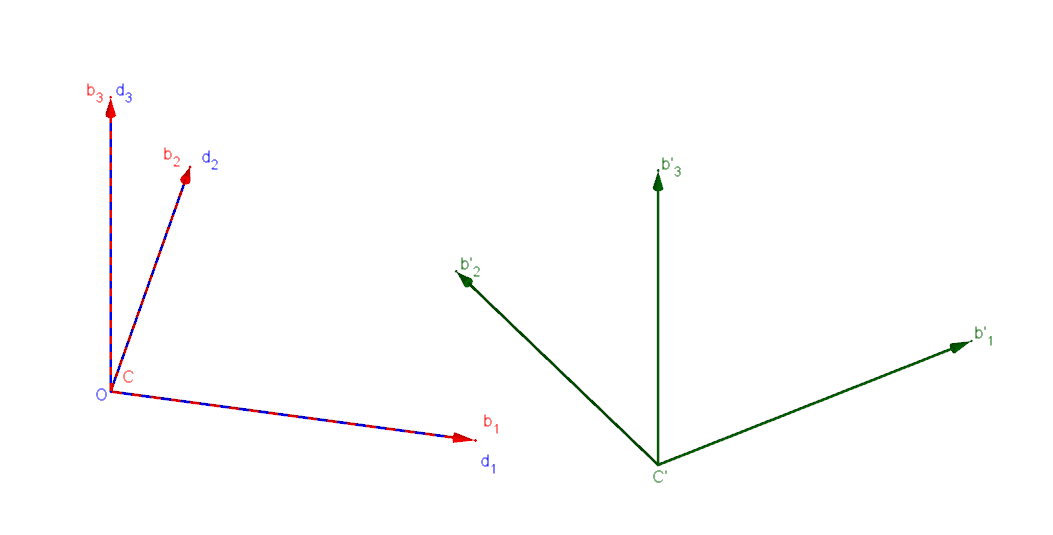
\includegraphics[width=.52\linewidth]{images/KS_Minimalbeispiel.png}
	\captionof{figure}{In Blau und Rot sind jeweils das Welt- und Kamerakoordinatensystem von Kamera eins zu sehen. In grün ist das gedrehte Koordiantensystem von Kamera 2 zu sehen.}
\end{minipage}\\ \\

\section{Vorgehen: Projektion eines Quaders in zwei verschieden transformierte Kameras}


Für die Stereokamerakalibrierung wird $C'$ relativ zur zu $C$ um einen Vektor \ensuremath{\vec{V'}} verschoben und anschließend um einen Winkel \ensuremath{\alpha} um die $b'_3$ Achse gedreht. Für die Rotation um \ensuremath{b'_3} wird eine Drehmatrix $D'$ aufgestellt.

\begin{gather}		
D'= 
\begin{pmatrix}
\cos(\alpha)&0&\sin(\alpha)\\
0&1&0\\
-\sin(\alpha)&0&\cos(\alpha)
\end{pmatrix}
\end{gather}

Um die Transformationsmatrix \ensuremath{R'}, welche die Rotation und die Translation von $C'$ beinhaltet, zu erhalten werden \ensuremath{D'} und \ensuremath{\vec{V'}} miteinander verrechnet.
\begin{gather}
\vec{V'}= 
\begin{pmatrix}
1&0&0&-v'_1\\
0&1&0&-v'_2\\
0&0&1&-v'_3			
\end{pmatrix}\\
R'=D'^T\cdot \vec{V'}\\
R'=		\begin{pmatrix}
\cos(\alpha)&0&-\sin(\alpha)\\
0&1&0\\
\sin(\alpha)&0&\cos(\alpha)
\end{pmatrix} 
\cdot
\begin{pmatrix}
1&0&0&-v'_1\\
0&1&0&-v'_2\\
0&0&1&-v'_3			
\end{pmatrix}\\
R'=
\begin{pmatrix}
\cos(\alpha)&0&-\sin(\alpha)&-v'_1\cos(\alpha)+v'_3\sin(\alpha)\\
0&1&0&-v'_2\\
\sin(\alpha)&0&\cos(\alpha)&-v'_1\sin(\alpha)-v'_3\cos(\alpha)\\
\end{pmatrix}
\end{gather}\\

Die entstandene Matrix \ensuremath{R'} beschreibt die Transformation $C'$ und somit auch die Transformation von Punkten des Koordinatensystems $(C,\beta)$ in $(C',\beta')$. Da $(C,\beta) = (O,\delta)$ ist, beinhaltet die Transformationsmatrix $R$ für $C$ weder eine Translation noch eine Rotation.

\begin{gather}
V=\begin{pmatrix}
0\\0\\0
\end{pmatrix}\\
	R = [I|V]\\
	R = \begin{bmatrix}
	1&&0&&0&&v_1\\
	0&&1&&0&&v_2\\
	0&&0&&1&&v_3
	\end{bmatrix}
\end{gather} 


\section{Berechnung der Projetkionsmatritzen }

Die Eckpunkte des Quaders $A_\delta,B_\delta,C_\delta,D_\delta,A'_\delta,B'_\delta,C'_\delta,D'_\delta$ sind bekannt. Neben den Eckpunkten des Quaders wird noch ein neunter Punkt $E_\delta$ außerhalb des Quaders platziert und zwar so, dass es zu keinen linearen Abhängigkeiten zwischen $E_\delta$ und den anderen Punkten kommt. So kann vermieden werden, dass die später aufgestellt Koeffizientenmatrix, zum berechnen der Fundamentalmatrix, einen Rang kleiner als acht bekommt und somit zwei linear unabhängige Lösungen ausgibt\cite{HZ}. Im Unterkapitel \nameref{sec:MinimalFun} wird nochmal genauer drauf eingegangen, was das für $F$ bedeutet. Fürs erste wird festgelegt, dass insgesamt neun Punkte sich in der Szene befinden. Um diese Punkte auf die Bildebenen $(I,\tau)$ und $(I',\tau)$ zu projizieren, müssen neben den Transformationsmatrizen $R$ und $R'$ noch die Kameramatrizen $K$ und $K'$ festgelget werden. 


\begin{gather}		
K =
\begin{bmatrix}
\zeta_{C}&0&0&0\\
0&\zeta_{C}&0&0\\
0&0&\zeta_{C}&0\\
0&0&1&0
\end{bmatrix}\\
K' =
\begin{bmatrix}
\zeta_{C'}&0&0&0\\
0&\zeta_{C'}&0&0\\
0&0&\zeta_{C'}&0\\
0&0&1&0
\end{bmatrix}
\end{gather}

Sind $R,R',K$ und $K'$ bekannt, können die Projektionsmatrizen $P$ und $P'$ berechnet werden. Vorher werden $R$ und $R'$ noch projektiv erweitert.


\begin{gather}
R=
\begin{bmatrix}
1&&0&&0&&v_1\\
0&&1&&0&&v_2\\
0&&0&&1&&v_3
\end{bmatrix}\\
P = K\cdot R \\
P =
\begin{bmatrix}
\zeta_{C}&0&0&0\\
0&\zeta_{C}&0&0\\
0&0&\zeta_{C}&0\\
0&0&1&0
\end{bmatrix}\\
P' = K' \cdot R'\\
P' =
\begin{bmatrix}
\zeta_{C'} \cos(\alpha)&0&\zeta_{C'} \sin(\alpha)&-\zeta_{C'} (v'_1\cos(\alpha)+v'_3\sin(\alpha) )&0\\
0&1&0&\zeta_{C'}-v'_2&0\\
\zeta_{C'}\sin(\alpha)&0&\zeta_{C'}\cos(\alpha)&-\zeta_{C'}(v'_1\sin(\alpha)+v'_3\cos(\alpha))\\
0&0&0&0&1
\end{bmatrix}
\end{gather}



\section{Transformation der Objektpunkte von Weltkoordinaten in Kamerakoordinaten}

Die 3D-Punkte $A_\delta,B_\delta,C_\delta,D_\delta,A'_\delta,B'_\delta,C'_\delta,D'_\delta, E_\delta$, werden um eine Homogene Komponenten erweitert und mit den Projektionsmatrizen \ensuremath{P} und \ensuremath{P2} zu, auf die Bildebenen $I$ und $I'$ projizierten, Punkten der Kamerakoordinatensysteme $(C,\beta)$ und $C',\beta'$ transformiert.

\begin{gather}		
Q_\beta =	
P \cdot	
\begin{bmatrix}
\begin{pmatrix}
\\A_\delta\\\\1
\end{pmatrix}&
\begin{pmatrix}
\\B_\delta\\\\1
\end{pmatrix}&
\begin{pmatrix}
\\C_\delta\\\\1
\end{pmatrix}&
\begin{pmatrix}
\\D_\delta\\\\1
\end{pmatrix}&
\begin{pmatrix}
\\A'_\delta\\\\1
\end{pmatrix}&
\begin{pmatrix}
\\B'_\delta\\\\1
\end{pmatrix}&
\begin{pmatrix}
\\C'_\delta\\\\1
\end{pmatrix}&
\begin{pmatrix}
\\D'_\delta\\\\1
\end{pmatrix}&
\begin{pmatrix}
\\E_\delta\\\\1
\end{pmatrix}
\end{bmatrix}\\
Q_{\beta'} =	
P' \cdot	
\begin{bmatrix}
\begin{pmatrix}
\\A_\delta\\\\1
\end{pmatrix}&
\begin{pmatrix}
\\B_\delta\\\\1
\end{pmatrix}&
\begin{pmatrix}
\\C_\delta\\\\1
\end{pmatrix}&
\begin{pmatrix}
\\D_\delta\\\\1
\end{pmatrix}&
\begin{pmatrix}
\\A'_\delta\\\\1
\end{pmatrix}&
\begin{pmatrix}
\\B'_\delta\\\\1
\end{pmatrix}&
\begin{pmatrix}
\\C'_\delta\\\\1
\end{pmatrix}&
\begin{pmatrix}
\\D_\delta'\\\\1
\end{pmatrix}&
\begin{pmatrix}
\\E_\delta\\\\1
\end{pmatrix}
\end{bmatrix}
\end{gather}

Die entstanden Bildebenenkoordinaten zur Basis der Kamerakoordintensysteme müssen dann wieder auf eine homogene Form gebracht werden, indem sie durch ihre jeweils letzte Komponenten dividiert werden. 


\begin{gather}
A_\beta = 
\begin{pmatrix}
b_1\\b_3\\ b_2\\\gamma
\end{pmatrix}
\leadsto A_\beta= 
\begin{pmatrix}
\frac{b_1}{\gamma}\\ \frac{b_3}{\gamma}\\ \frac{b_2}{\gamma}\\ \frac{\gamma}{\gamma}
\end{pmatrix}
\leadsto A_\beta =
\begin{pmatrix}
\hat{b_1}\\
\hat{b_2}\\
\hat{b_3}\\
1
\end{pmatrix}\\
\simeq
\begin{pmatrix}
t_1\\
t_2\\
\zeta\\
1
\end{pmatrix}
\end{gather}\\

Der in Gleichung 4.18 verwendete Kamerapunkt $A_\beta$ liegt direkt auf der Bildebene $I$, was durch die Projektionsmatrix $P$ bedingt wurde. Die Tiefenkomponente entspricht deshalb nach der homogenisierung des Punktes dem Wert $\zeta$, welcher den Abstand $\overline{IC}$ beschreibt. Um die 3D-Kamerapunkte in 2D-Bildebenenpunkte zur Basis $(I,\tau)$ mit $\tau = (t_1,t_2)$ und für $C'$ entsprechend $(I',\tau')$ mit $\tau' = (t'_1,t'_2)$ umzuwandeln, muss lediglich der Tiefenwert $\zeta$ entfernt und durch die Homogene Komponenten ersetzt werden. In Abbildung 4.4, sind die entstehenden Abbildilder auf die jeweiligen Bildebenen in 2D-Bildebenenkoordinaten $(I,\tau)$ und $(I',\tau')$ zu sehen.

\begin{gather}
	 A_\beta =
	\begin{pmatrix}
	\hat{b_1}\\
	\hat{b_2}\\
	\hat{b_3}\\
	1
	\end{pmatrix}
	\simeq
	\begin{pmatrix}
	t_1\\
	t_2\\
	\zeta\\
	1
	\end{pmatrix}\\
	\leadsto A_\tau = 
	\begin{pmatrix}
	t_1\\
	t_2\\
	1
	\end{pmatrix}\\
\end{gather}



\begin{minipage}{\linewidth}
	\centering
	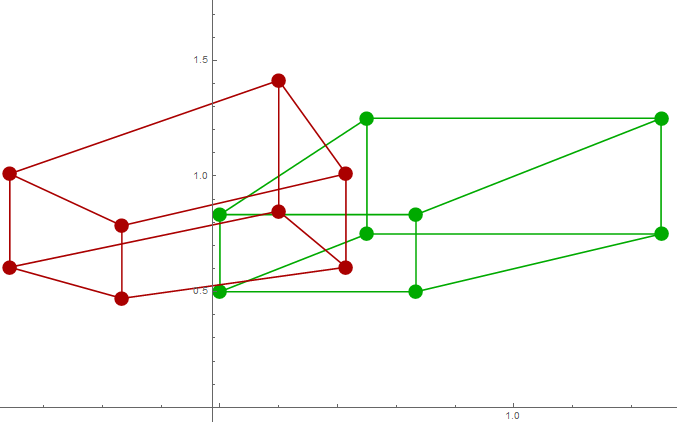
\includegraphics[width=0.8\linewidth]{images/QuadrateMinimalBeispiel.png}
	\captionof{figure}{Grün zeigt den Quader welcher auf $I$ von $C$ abgebildet wird. Das größere Quadrat sind die vorderen Punkte \ensuremath{A,B,C,D}, das kleinere Quadrat sind die hinteren Punkte \ensuremath{A',B',C',D'}. Der Punt $E$ ist weiter weg von den Abbildungen und deshalb auf dieser Abbildung momentan nicht zu sehen. Rot zeigt denselben Quader auf $I'$ von $C'$ abgebildet.}
\end{minipage}\\
%\section{Berechnung der projizietrten Punkte auf den beiden Bildebenen}
%
%Um die 3D-Kamerakoordinaten auf die 2D-Bildebene zu Projizieren muss man lediglich die Tiefeninformation der Punkte \ensuremath{PK1} und \ensuremath{PK2} entnehmen und durch die homogene Koordinate ersetzen. Die folgende Gleichung zeigt ein Beispiel dazu 
%
%\begin{gather}
%aK2 =
%\begin{pmatrix}
%\tilde{x}\\
%\tilde{y}\\
%z\\
%1
%\end{pmatrix} 
%\leadsto aBK2 = 		
%\begin{pmatrix}
%\tilde{x}\\
%\tilde{y}\\
%1
%\end{pmatrix}
%\end{gather}

\section{Umrechnung von Bildebenenkoordinaten in Sensorkoordinaten}

Für die Umrechnung der Bildebenenkoordinaten $A_\tau,B_\tau,C_\tau,D_\tau,A'_\tau,B'_\tau,C'_\tau,D'_\tau, E_\tau$ und $A_{\tau'},B_{\tau'},C_{\tau'}$, $D_{\tau'},A'_{\tau'},B'_{\tau'},C'_{\tau'},D'_{\tau'}, E_{\tau'}$ in Sensorkoordianten $(S,\sigma)$ mit $\sigma = (\vec{u},\vec{v})$, muss der sogenannte Pixelpitch des Sensors bekannt sein. Für das Minimalbeipiel wird ein PixelPitch von 1 angenommen. Die Bilebenenkoordinaten werden so 1:1 in die Sensorkoordinaten umgesetzt. In Realbeispielen ist dies aber eher selten der Fall. Die Sensorkoordinaten sind im normalfall in Pixeleinheiten gegeben und werden für die Berechnung der Fundamentalmatrix benötigt.

\begin{gather}
\sigma = (\vec{u},\vec{v})\\	
\vec{u} = u_1t_1+u_2t_2\\
\vec{v} = v_1t_1+v_2t_2\\
S_\sigma = I_\tau +p_{x\tau}+p_{y\tau}\\
(\vec{u},\vec{v}, S_\sigma)=(t_1,t_2,I\tau)\cdot
\begin{bmatrix}
u_1&u_2&z_1\\
v_1&v_2&z_2\\
0&0&1
\end{bmatrix}	\\
M = 	
\begin{bmatrix}
u_1&u_2\\
v_1&v_2
\end{bmatrix}
\end{gather}

Mit dem Berechnen der Sensorkoordinaten ist der Aufba der Szene vollendet. Das Ergebnis sind zwei Bilder des Quaders von zwei verschiedenen Kameras mit momentan noch gleicher Auflösung. In den nächsten Schritten soll nun anhand der Bildpunkte eine Rekonstruktion der exterenen Kameraparameter und eine Rekonstruktion der synthtischen Szene folgen. Die intrinsischen Parameter werden in dieser Arbeit immer als bereits bekannt festgelegt. \textcolor{red}{(Hier vllt noch erwähnen, dass die calibrierung der inneren Kameraparameter in einer anderen Arbeit behandelt wurde, außerdem kann hier auch eine getrennt kalibrierung beider kameras durchgeführt werden) }

\section{Fundamentalmatrix und der eight-Point-Algorithmus}
\label{sec:MinimalFun}




Nachdem nun die Bildkoordinaten in Pixel des Quaders auf den Bildern der beiden Kameras bekannt sind, kann nun die eigentliche Rekonstruktion der externen Kameraparameter und die 3D-Szenenrekonstruktion beginnen. Der erste Schritt beinhaltet die ermittlung der Fundamentalmatrix $F$ mit den korrespondierenden Bildpunkten der beiden Kamerabilder mit Hilfe des sogenannten  \textit{8-Point-Algorithms}. Der \textit{8-Point-Algorithm} ist eine lineare Technik die angewandt wird, um die essentielle Matrix und die Fundamentalmatrix aus  $n \geq 8$ Punkten zu schätzen \cite{Zhang2014,HZ}. Der Algorithmus benötigt $n \geq 8$ Punkte, um ein valides eindeutiges Ergebnis zu liefern \cite{HZ,Ferid}.Es besteht noch die Möglichkeit den \textit{7-Point-Algorithm} anzuwenden, welcher nach dem selben Prinzip wie sein Verwandter \textit{8-Point-Algorithm} verfährt, jedoch kein eindeutiges Ergebnis liefert. Mit sieben Punkten bekommen wir als Lösung zwei linear unabhängige Kerne als Lösung der zuvor aufgestellten Koeffizientenmatrix mit welchen für ein eindeutiges Ergebnis noch weiter verfahren werden muss\cite{HZ,Ferid}. Die aufgestellte Koeffizientenmatrix, hat im Fall des \textit{7-Point-Algorithm} nämlich nur den Rang 7\cite{HZ}. In Für Schätzung von $F$ wurde in diesem Minimalbeispiel und auch später in Realbeispiel der \textit{8-Point-Algorithm} verwendet. Im Falle des Minimalbeispiels, wurde mit einem zusätzlichen neunten Punkt auch noch dafür gesorgt, dass die aufgestellte Koeffizientenmatrix auch den Ran 8 besitzt. Somit kann, wie bei der Bestimmung der Homographie, einfach der Nullraum der Koeffizientenmatrix bestimmt werden, welcher die Einträge der 3x3-Matrix von $F$ liefert\cite{HZ}. Besitz die Koeffizientenmatrix $A$ einen Rang größer 8, so wird auch hier mit einem \textit{least-square}- Verfahren, mit Hilfe der Singulärwertszerlegung, angewendet werden, so dass $||A \cdot f||$ minimal wird. $f$ ist der Singulärvektor, welcher mit dem kleinsten Singulärwert korrespondiert\cite{HZ}. Die genaue Abfolge des Verfahrens, wird im Kapitel \nameref{sec:realFun} genauer aufgezeigt. Da im Minimalbeispiel der Rang 8 der Koeffizientenmatrix erzwungen wurde, reicht es vorerst den Nullraum zu bestimmen. Die Koeffizientenmatrix wird aus dem Ausdruck \textit{epipolar-constraint} in Gleichung 4.29 aufgestellt. Der ermittelte Kern und alle seine Vielfache sind mögliche Lösungen für $F$\cite{HZ,Ferid}. 

\begin{gather}
{m'}_{\sigma'}^T \cdot F \cdot m_\sigma =0\\
F=\begin{bmatrix}
f_{11}&f_{122}&f_{13}\\
f_{21}&f_{22}&f_{23}\\
f_{31}&f_{32}&f_{33}
\end{bmatrix}\\
\begin{bmatrix}
x'_n&y'_n&1
\end{bmatrix} 
\cdot
\begin{bmatrix}
f_{11}&f_{122}&f_{13}\\
f_{21}&f_{22}&f_{23}\\
f_{31}&f_{32}&f_{33}
\end{bmatrix}
\cdot
\begin{bmatrix}
x_n\\y_n\\1
\end{bmatrix} =0\\
f_{11}x_nx'_n+f_{12}y_nx'_n+f_{13}x'_n+f_{21}x_ny'_n+f_{22}y_ny'_n+f{23}y'_n+f_{31}x_n+f_{32}y_n+f_{33} =0\\
(x_nx'_n,y_nx'_n,x'_n,x_ny'_n,y_ny'_n,y'_n,x_n,y_n,1)\cdot f =0\\
\begin{bmatrix}
x_1x'_1&y_1x'_1&x'_1&x_1y'_1&y_1y'_1&y'_1&x_1&y_1&1\\
x_2x'_2&y_2x'_2&x'_2&x_2y'_2&y_2y'_2&y'_2&x_2&y_2&1\\
.&.&.&.&.&.&.&.&.\\
.&.&.&.&.&.&.&.&.\\
.&.&.&.&.&.&.&.&.\\
x_nx'_n&y_nx'_n&x'_n&x_ny'_n&y_ny'_n&y'_n&x_n&y_n&1
\end{bmatrix}
\cdot 
\begin{pmatrix}
f_{11}\\f_{12}\\f_{13}\\f_{21}\\f_{22}\\f_{23}\\f_{31}\\f_{32}\\f_{33}
\end{pmatrix}
= 0
\end{gather}


\section{Epipole und Epipolargeraden}

Mit Hilfe der Fundamentalmatrix und dem Wissen über die Epipolargerometrie, kann man die Epipole \ensuremath{e} und \ensuremath{e'}, sowie die Epilolargeraden \ensuremath{l} und \ensuremath{l'} ermitteln.


% Im ersten Abschnitt wird die ermittlung mit Hilfe der Fundamentalmatrix aufgezeigt und in Kapitel 1.2.1 wird nochmal drauf eingegangen und aufgezeigt, wie sich die Epipolarlinien und Epipole geometrisch Konstruieren lassen. Mit der Fundamentalmatrix lassen sich die Epipolargerade folgendermaßen berechnen\\



\begin{gather}
l' = F \cdot m\\
l = F^T \cdot m'
\end{gather}\\

\ensuremath{l'} ist die zu \ensuremath{m} korrespondierende Epipolargerade. \ensuremath{l} ist die zu \ensuremath{m'} korrespondierende Epipolargerade. Zu Berechnung des Epipols \ensuremath{e} muss der Rechte Kern von $F$ ermitteln werden und für den Epipol \ensuremath{e'} brauchen wir den linken Kern. Die Abbiludng 4.5 zeigt, dass Ergebnis der Epipole im Minimalbeispiel. 

%
%Um diesen zu bekommen ermitteln wir wie bekannt den Kern aber diesmal von \ensuremath{F^T} statt \ensuremath{F}. 

\begin{minipage}{\linewidth}
	\centering
	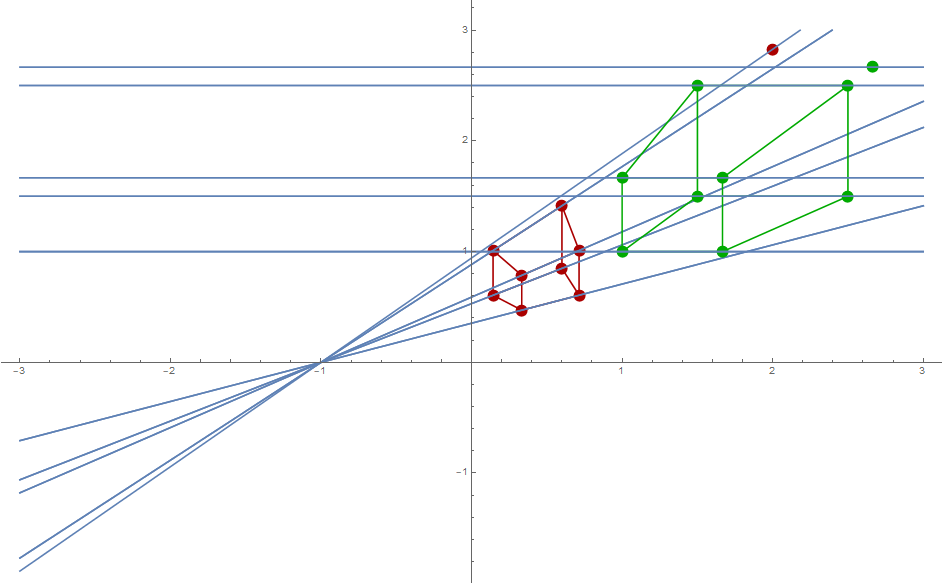
\includegraphics[width=1.\linewidth]{images/Epipole_Epipollinien.png}
	\captionof{figure}{Die blauen Geraden zeigen die jeweiligen Epipolargeraden. Die vom roten Quader schneiden sich bei -1 im Epipol $e'$ . Die Epipolargeraden vom grünen Quader schneiden sich im Epipol $e'$ im Unendlichen, weshalb die Epipolarlinien Parallel zueinadner verlaufen.}
\end{minipage}\\ \\

\subsection{Geometrische Konstruktion der Epipole und der Epipolarlinien}


Die Vorgehensweise zur Ermittlung der Epipole und der Epipolgeraden ist zwar schnell aber zur verdeutlichung der geometrischen Beziehungen untereinander wird nochmal eine rein geoemtrische Konstruktion der Epipole und der Epipolargeraden durchgeführt. Im nachfolgenden Beispiel wird der Epipol \ensuremath{e'} geometrisch konstruiert. Umrechnung von allen Punkten in ein gemeinsames Koordinatensystem, zum Beispiel in $(C,\beta)$. Für die Konstruktion der Epipole wird die BasisLinie $B = C'_\beta - C_\beta$, ein Bildebenenpunkt $A_{C'\beta}$ auf $I'$ und die Position von $I'$ selbst benötigt.


\begin{gather}
B = C'_\beta + t\cdot (C'_\beta-C_\beta)
\end{gather}

Um den Epipol zu ermitteln wird der Schnittpunkt der Gerade $B$ mit der Bildebenen $I'$ von $C'$ benötigt. Die Bildebene $I'$ wird in einer Ebenen Normalenform dargestellt. Als Bildebenenpunkt wird $A_{C'\beta}$ von $I'$ von $C'$ gewählt.


\begin{gather}
\vec{n_0}\cdot[\vec{x}-A_{C'\beta}]
\end{gather}


%(HIER WEITER SCHREIBEN)
%Nehmen wir das bereits bekannte Beispiel von vorhin, in welchem die Kamera 2 entlang der positiven \ensuremath{e_1} verschoben und um 45° um die \ensuremath{e_2}-Achse gedreht wurde, so ist der normalen Vektor der Bildebene aus sicht der Weltkoordinaten \ensuremath{\vec{n_0} = \begin{pmatrix}
%		-1\\0\\-1
%\end{pmatrix}}. Für die Ebene brauchen wir nun noch einen Punkt welcher auf ihr liegt. In unserem Beispiel nehmen wir als Aufpunkt \ensuremath{\vec{a}} den Punkt \ensuremath{a} in Bildkoordinaten \ensuremath{aBK2} der 2. Kamera und rechnen diesen in Weltkoordinaten zurück. Wir brauchen also die nicht-transponierte Rotation \ensuremath{R} welche lautet:
%
%\begin{gather}
%R=\begin{pmatrix}
%\cos{\alpha}&0&\sin{\alpha}\\
%0&1&0\\
%-\sin{\alpha}&0&\cos{\alpha}
%\end{pmatrix}
%\end{gather}
%
%Des Weiteren brauchen wir den verschiebe Vektor \ensuremath{\vec{v} = \begin{pmatrix}
%		v_1\\v_2\\v_3
%\end{pmatrix}},welcher mit \ensuremath{R} verrechnet wird.
%
%
%\begin{gather}
%\begin{pmatrix}
%\cos{\alpha}&0&\sin{\alpha}\\
%0&1&0\\
%-\sin{\alpha}&0&\cos{\alpha}
%\end{pmatrix}
%\cdot
%\begin{pmatrix}
%v_1\\v_2\\v_3
%\end{pmatrix}
%=
%\begin{pmatrix}
%v_1\cos{\alpha}+v_3\sin{\alpha}\\
%v_2\\
%-v_1\sin{\alpha}+v_3\cos{\alpha}
%\end{pmatrix}\\
%\leadsto D =
%\begin{bmatrix}
%\cos{\alpha}&0&\sin{\alpha}&v_1\cos{\alpha}+v_3\sin{\alpha}\\
%0&1&0&v_2\\
%-\sin{\alpha}&0&\cos{\alpha}&-v_1\sin{\alpha}+v_3\cos{\alpha}\\
%0&0&0&1
%\end{bmatrix}
%\end{gather}\\
%
%Matrix \ensuremath{D} wird dann mit Punkt \ensuremath{aBK2} multipliziert und wir bekommen den Punkt \ensuremath{aBK2} in Weltkoordinaten \ensuremath{aWK2}. Die Normalengleichung ist somit komplett aufgestellt. um auf die Koordinatengleichung zu kommen werden die Skalare einfach ausmultipliziert. 
Um den Schnittpunkt der Gerade $B$ mit der Ebene $I$ zu berechnen, wird die Gerade $B$ in die Ebenengleichung eingesetzt und es wird ein Wert für $t$ ermittelt. 
\begin{gather}
\vec{n_0}\cdot \vec{x} - \vec{n_0}\cdot \vec{a}\\
\end{gather}

Danach wird die Geradengleichung \ensuremath{BaseLine} in die Ebenengleichung \ensuremath{ImagePlane} eingesetzt und es wird ein Wert für \ensuremath{t} ermittelt. Der berechnete Wert für $t$ wird dann wiederum in $G$ eingesetzt und das Ergebnis ist der Epipol \ensuremath{e'_\beta}. Dieser kann dann wieder über bereits bekannte Transformationen in die Sensorkoordinaten von $(S',\sigma)$ bezüglich $C'$ überfürht werden.

\begin{gather}
e'_\sigma=P'.e'_\beta
\end{gather}

Für die Epipolarlinien $l'_{\sigma'}$ durch $e'_{\sigma'}$, müssen einfach Geradengleichungen eines Sensorpunktes, beispielsweise $A_{\sigma'}$, durch $e_{\sigma'}'$ aufgestellt werden. Die entstandenen Linie ist dann die Epipolarlinie zum Punkt $A_{\sigma'}$ und gleichzeitig die korrespondierende Epipoloarlinie zum Sensorpunkt $A_\sigma$ von $I$ von $C$.

\begin{gather}
	g:= A_{\sigma'} +t \cdot (A_{\sigma'}-e'_{\sigma'})
\end{gather}

\section{Essentiellen Matrix}


Für die Rekonstruktion der externen Kameraparameter, gibt es verschiedene Ansätze \cite{HZ}. Es ist zum einen Möglich, ohne Vorwissen der Kameramatrizen oder Transformationsmatrizen, aus der Fundamentalmatrix über den sogenannten \textit{Stratified approach} die komplette Projektionsmatrix $P$ und $P'$ zu ermitteln, jedoch ohne weitere Informationen über die 3S-Szene nur bis zu einem Projektiven Vieldeutigkeit\cite{HZ}. Da in dieser Arbeit davon ausgegangen wird, dass die Kameras zuvor einzeln Kalibriert wurden und die intrinsischen Kameraparameter bereits bekannt sind(hier vllt vorherige Arbeit erwähnen), wird für die Rekonstruktion der externen Kameraparameter ein Ansatz verfolgt, in welchen die essentielle Matrix zum Einsatz kommt. Die essentielle Matrix ist eine Spezialform der Fundamentalmatrix und beschreibt den \textit{epipolar constraint}, im  kalibrierten Fall, zwischen den normalisierten Bildkoordinaten $\hat{m_\sigma}$ und $\hat{m}'_{\sigma'}$\cite{HZ,Elements,ZZGXr,Zhang2014,Ferid}. 


\begin{gather}
\hat{m}'^T_{\sigma'}.E.\hat{m}_\sigma = 0
\end{gather}\\ 

Ist die Fundamentalmatrix $F$ bereits ermittelt worden und die Kameramatrizen $K$ und $K'$ bekannt, kann die essentielle Matrix wie im Kapitel \nameref{sec:epipolar} aus $F$ berechnet werden. Die essentielle Matrix ist eine Fundamentalmatrix, welche zu einem paar normalisierten Projektionsmatrizen $P$ mit $P = [I|0]$ und $P'$ mit $P'= [R'|V']$ korrespondierend ist\cite{HZ,Zhang2014,ZZGXr,Ferid}. Um eine Projektionsmatrix $P'=K'[R'|V']$ auf die normalisierte Form zu bringen, müssen die intrinsischen Parameter für $K'$ bekannt sein. 

\begin{gather}
	m'_{\sigma} = P' \cdot M_\delta\\
	m'_{\sigma} = K'[R'|V'] \cdot M_\delta\;\; | \cdot K'^{-1}\\
	K'^{-1} \cdot m'_{\sigma} = K'^{-1} \cdot K'[R'|V'] \cdot M_\delta\\
	\hat{m}'_{\sigma} = [R'|V'] M_\delta
\end{gather}

$M_\delta$ ist der ein Objektpunkt im 3D-Raum, welcher mit $P'$ zum Sensorpunkt $m'_{\sigma'}$ abgebildet wird. Nach der Normalisierung, wird $\hat{m}'_{\sigma}$ als normalisierte Koordinat bezeichnet und die entstandene Projektionsmatrix $P' = [R'|V']$ als normalisierte Projektionsmatrix\cite{HZ,Ferid}. Die essentielle Matrix $E$ beschreibt dann die korrespondenz zwischen den korrespondierenden normalisierten Koordinaten  $\hat{m_\sigma}$ und $\hat{m}'_{\sigma'}$ wie in Gleichung 4.43 gezeigt. Um $E$ aus $F$ zu gewinnen, werden die Kameramatrizen $K$ und $K'$ mit $F$ multipliziert. Zu Erinnerung im Kapitel \nameref{sec:epipolar} wurde genau diese Beziehung zwischen $E$ und $F$ in den Gleuchungen 3.98 bis 3.101 aufgeführt. 


\begin{gather}
E = K'^T.F.K
\end{gather}

Das Ergebnis dieser der Gleichung 4.48 und alle deren Vielfache, sind mögliche Lösungen für die essentielle Matrix. Wie die Fundamentalmatrix muss auch die essentielle Matrix einen Rang von 2 haben. Des Weiteren darf eine 3x3-Matrix nur dann als essentielle Matrix bezeichnet werden, wenn die Singulärwerte, welche durch eine Singulärwertszerlegung ersichtlich werden, bestimmte Merkmale aufweisen. So müssen zwei der drei Singulärwerte gleich und die dritte null sein\cite{HZ}. Des Weiteren muss für die Dtermintante gelten, dass $det(E) = 0$ ist und die Quadratwurzel der Eigenwerte müssen wieder die Singulärwerte ergeben. Die essentielle Matrix kann, wie die Fundamentalmatrix auch, über den \textit{8-Point-Algorithm} ermittelt werden. Jedoch müssen auch hier die intrinsischen Kameraparameter $K$ und $K'$ bekannt sein. Die korrespondierenden Punkte, werden in normalisierte Bildkoordinaten umgerechnet und dann in eine Koeffizientenmatrix gleich der Matrix in Gleichung 4.34 eingetragen. Danach kann $E$ entweder über die Bestimmung des Kerns oder, im Falle von Realen Bilddaten, dem \textit{least-square}- Verfahren geschätzt werden\cite{HZ,Ferid}.

%\subsection{Ermitteln der Essentiellen Matrix mit normierten Bildkoordinaten und dem 8-Point-Algorithm}
%
%Im vorherigen Abschnitt haben wir bereits die normierten Bildebenenkoordinaten berechnet. Um die essentielle Matrix mit dem 8-Point-Algorithm zu bestimmen, verfährt genau so wie bei der Bestimmung der Fundamentalmatrix nur verwendet man statt den Sensorkoordinaten die normierten Bildebenenkoordinaten.\\ (vgl Hartley and Zisserman, O. Schreer)
%
%Um herauszufinden, ob die errechnete Matrix den Kriterien einer Essentiellen Matrix entspricht gilt folgendes zu überprüfen.
%
%\begin{itemize}
%	\item Zwei der Singulärwerte und der Eigenwerte der Essentiellen Matrix müssen gleich und von null verschieden sein.
%	\item Die Quadratwurzel der Eigenwerte muss die Singulärwerte ergeben
%	\item Der Rang der Matrix muss zwei sein
%\end{itemize}

\section{Exterenen Kameraparameter mit essentieller Matrix}


Mit der essentiellen Matrix ist es möglich die Transformationsmatrize $R'$ zu ermitteln. Es wird davon ausgegangen, dass für $R$ gilt $R = [I|0]$. Die aus $E$ ermittelte Matrix $R'$ beschreibt dann die Transformation von $C'$ relativ zu $C$\cite{HZ,Ferid}. Um die externen Kameraparameter zu bestimmen, wird zunächst die essentielle Matirx \ensuremath{E} mit Hilfe der Singulärwertszerlegung in drei Matrizen zerlegt. 

\begin{gather}
E = U\Sigma V^T
\end{gather}

Die Singulärwerte befinden sich in der mittleren Matrix $\Sigma = diag(\sigma_1,\sigma_2,\sigma_3)$ wieder. Damit die Matrix $E$ sich essentielle Matrix nennen darf, muss für zwei der Diagonaleinträge für die Singulärwerte gelten das $\sigma_1 = \sigma_2$ und für $\sigma_3$ muss dann dementsprechend gelten, dass $\sigma_3=0$. Sollten die Singulärwerte diesen Bedingungen nicht entsprechen, so wird ein so genannten \textit{singularity-constraint}, der Form $\Sigma = diag(\frac{\sigma_1+ \sigma_2}{2},\frac{\sigma_1+\sigma_2}{2},0)$, erzwungen\cite{HZ}. Im Minimalbeispiel kommt es auf Grund der eigens erstellten Bildpunkte zu keinen Bildfehlern, wie im Realbeispielen. Deswegen ist der \textit{singularity-constraint} nicht notwendig, da die Bedingungen für $E$ erfüllt sind.\\

Ein wichtiges Detail, was sich später auch auf die vier möglichen Ergebnisse für $P$ auswirkt, ist noch zu beachten. Zum einen sollte einem bewusst sein, dass die Zerlegung der essentiellen Matrix keine eindeutige Lösung hervorbringen muss. Für $E$ muss gelten, dass $\text{det}(E) = 0$ ist. Es wird also vorausgesetzt, dass die Determinante der aus der $SVD$ gewonnen Matrizen $UV^T = 1$ ist. Angenommen aus der $SVD$ von $E$ ergibt sich für die Determinanten von $UV^T = -1$, so können die Determinanten der Matrizen $U$ und $V$ getrennt voneinander bestimmt werden. Sollte $\text{det}(U)=-1$ oder $\text{det}(V)=-1$ oder beides zusammen der Fall sein, so kann die jeweilige Matrix einfach mit $-1$ multipliziert werden. $E$ setzt sich zusammen aus einer Rotationsmatrize $R$ und einer schiefsymmetrischen Matrix $S$.

\begin{gather}
E=[v]_xR\\
S =[v]_x\\
E=SR
\end{gather}

Zur Schätzung von $S$ und $R$ werden des Weiteren die schiefsymmetrische Matrix \ensuremath{W} und die Blockdiagonale Matrix \ensuremath{Z} eigeführt\cite{HZ}. Mit diesen Matrizen lassen sich die gesuchten $R$ und $S$ für $C'$ rekonstruieren, jedoch nur bis zu einer gewissen Skaleninvarianz\cite{HZ,Ferid}.


\begin{gather}
W = \begin{pmatrix}
0&-1&0\\
1&0&0\\
0&0&1
\end{pmatrix} \;\;\;
Z=
\begin{pmatrix}
0&1&0\\
-1&0&0\\
0&0&0
\end{pmatrix}
\end{gather}

Mit dem, je nach dem leicht modifizierten, Ergebnis der $SVD$ von \ensuremath{E} lassen sich nun jeweils zwei mögliche Lösungen für $S$ und $R$ aufstellen.


\begin{gather}
S_1 = -UZU^T \;\;\;\; R_1 = UW^TV^T\\
S_2 = UZU^T \;\;\;\; R_2 = UWV^T
\end{gather}\\


Um sicher zu gehen, dass es sich bei \ensuremath{R_1} und \ensuremath{R_2} auch um gültige Rotationsmatrizen handelt, kann eine Probe durchgeführt werden. Zum einen muss \ensuremath{R\cdot R^T=I_{3x3}} sein. \ensuremath{I_{3x3}} bezeichnet in diesem Fall die 3x3-Einheitsmatrix. Des Weiteren kann man überprüfen, ob die Determinante \ensuremath{det(R_1) = 1} ist. Ist die Determinante = -1, so ist die Rotation für ein Rechtsdrehendes System, ist die Determinaten = -1, so handelt es sich um ein linksdrehendes System\cite{HZ}. $S_1$ und $S_2$ sind jeweils schiefsymmetrische Matrizen aus welchen, jetzt noch zwei Lösungen für $v$ finden lassen müssen\cite{HZ}. 

\begin{gather}
St = [v]_\times \cdot v = v \times v
\end{gather} 

Um $v$ zu ermitteln muss also lediglich der Kern von $S_1$ und $S_2$ gefunden werden. Die jeweilgen Ergebnisse für $v_1$ und $v_2$ sind bis auf ihre Vorzeichen die selben.

 Die externen Kamerparameter lassen sich wie gesagt nur bis zu einem Skalierungsfaktor genau bestimmen. Die Rotationen $R$ ist von dieser Skaleninvarianz nicht betroffen, es betrifft nur den Translationsvektor $\vec{v}$. Wie mit der Skaleninvarianz weiter Verfaheren wird, wird im nachfolgenden Abschnitt der Szenenrekonstruktion durch Triangulierung noch aufgeführt. Letztendlich können, für die Rekonstruktion der externen Kameraparameter vier Lösungen für $P$ gefunden werden.\cite{HZ,Ferid}. $\lambda v$ heißt dabei, dass sowohl $v$ also auch alle Vielfache von $v$, Lösungen sein können, was durch die Skaleninvarianz der Lösung bedingt ist\cite{HZ,Ferid}. 

\begin{gather}
P = [UWV^T|+\lambda v] \;\;\; \textit{oder} \;\;\;[UW^TV^T|+\lambda v]\\
\textit{oder}\;\;\; [UWV^T|-\lambda v] \;\;\; \textit{oder} \;\;\;[UW^TV^T|-\lambda v]
\end{gather}

\begin{figure}[!htb]
	\minipage{0.52\textwidth}
	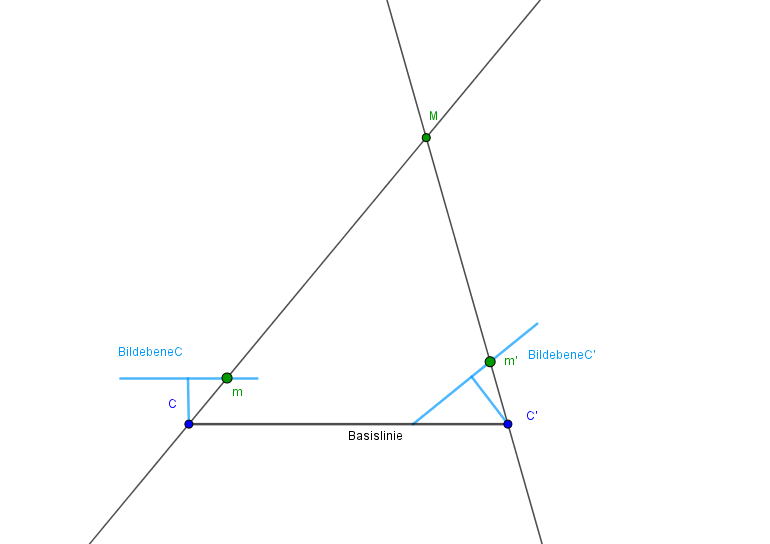
\includegraphics[width=\linewidth]{images/P_Solution_one.png}
	%	\caption{A really Awesome Image}
	\label{fig:awesome_image1}
	\endminipage\hfill
	\minipage{0.52\textwidth}
	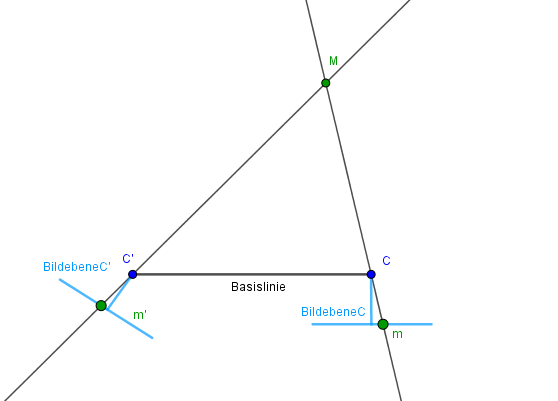
\includegraphics[width=\linewidth]{images/P_Solution_two.png}
	%	\caption{A really Awesome Image}
	\label{fig:awesome_image2}
	\endminipage\hfill
\end{figure}
\begin{figure}[!htb]
	\minipage{0.52\textwidth}
	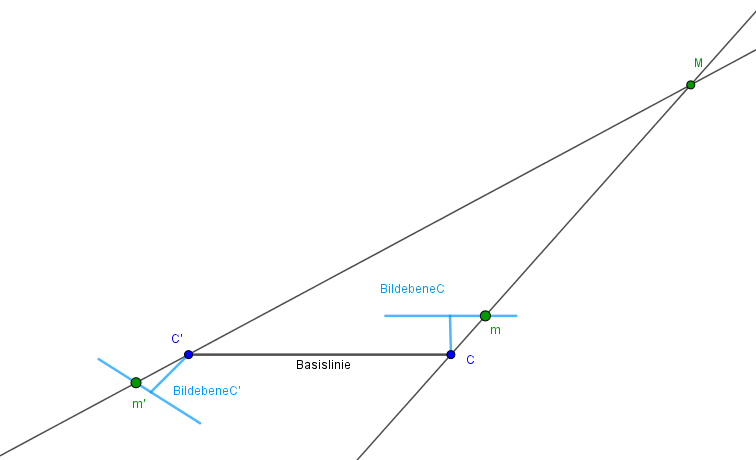
\includegraphics[width=\linewidth]{images/P_Solution_three.png}
	%	\caption{A really Awesome Image}
	\label{fig:awesome_image1}
	\endminipage\hfill
	\minipage{0.52\textwidth}
	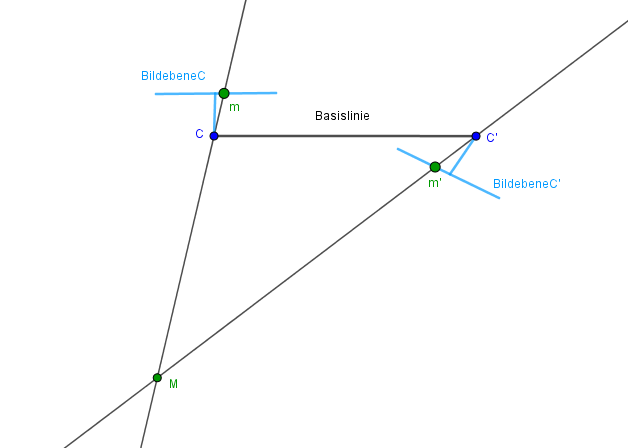
\includegraphics[width=\linewidth]{images/P_Solution_four.png}
	%	\caption{A really Awesome Image}
	\label{fig:awesome_image2}
	\endminipage\hfill
	\caption{Anordnung der Kameras bei den vier verschiedenen Lösungen für $P$}
\end{figure}
\pagebreak

\section{Szenenrekonstruktion durch Triangulation}


Unter Triangulierung versteht man das Rekonstruieren der 3D-Szenenpunkte durch Schnittpunktberechnung derjenigen Geraden, welche durch die jeweiligen Projektionszentren der Kameras und deren korrespondierenden Bildpunkte auf deren Bildebenen gehen, so dass sich ein Dreick bildet.\\


\begin{minipage}{\linewidth}
	\centering
	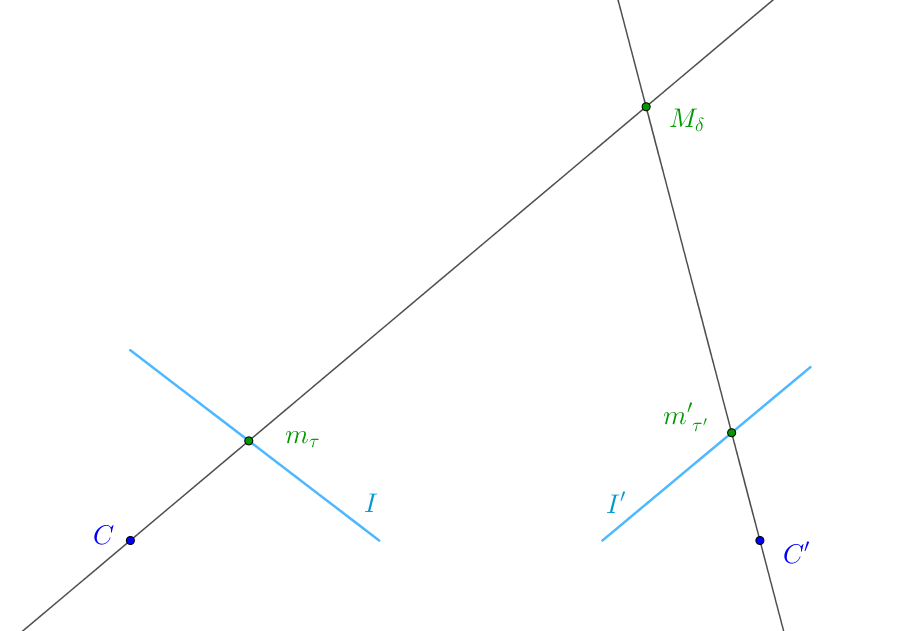
\includegraphics[width=0.8\linewidth]{images/optimaleTriangulierung.png}
	\captionof{figure}{Optimale Triangulierung: Beide Geraden Treffen sich in einem Punkt im 3D-Raum} 
\end{minipage}\\ \\


Da das Minimalbeispiel mit reinen Daten arbeitet, ist damit garantiert, dass die Linien sich in einem Schnittpunkt treffen. Anders hingegen wäre es in einem realen Beispiel mit korrespondierenden Punkten, welche Beispielsweise über einen \textit{SURF}- Algorithmus detektiert wurden\cite{Mandun}. In Realbildern, können Bildfehler wie beispielsweise Rauschen nicht vermieden werden, des Weiteren können korrespondierende Punkte nicht immer exakt auf den Pixel genau bestimmt werden. Diese Fehler führen dazu, dass wenn ein Schnittpunkt der Geraden durch die vermeintlichen korresponiderenden Punkte nicht gefunden werden kann, da die Geraden sich sehr wahrscheinlich nicht in einem Punkt treffen werden\cite{Mandun,HZ}. 


\begin{minipage}{\linewidth}
	\centering
	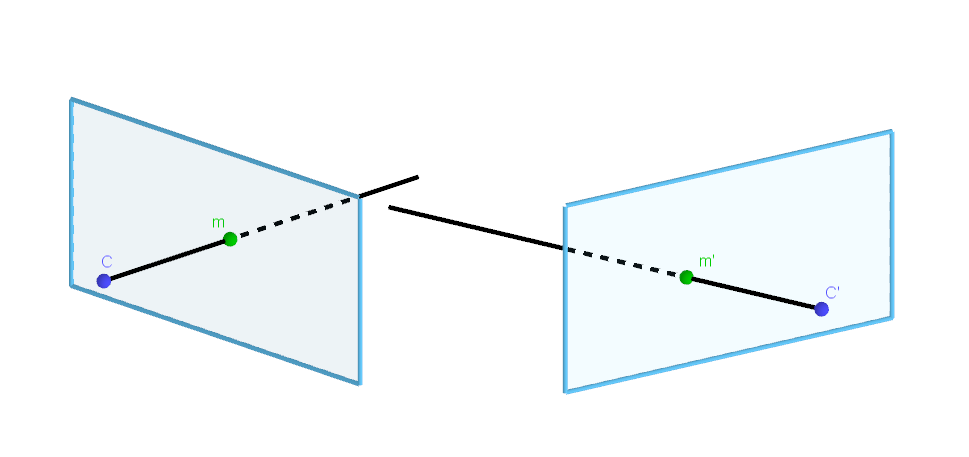
\includegraphics[width=0.8\linewidth]{images/problemTriangulation.png}
	\captionof{figure}{Durch Ungenauigkeiten in der korrespondierenden Punkte, verfehlen sich die Linien und es kommt zu keinem Schnittpunkt} 
\end{minipage}\\ 

Für diese Fälle gibt es mehrere Näherungsverfahren, wovon eines, im Kapitel \nameref{sec:sampson}, im Realbeispiel eingeführt wird\cite{HZ}. In diesem Minimalbeispiel tritt der optimale Fall ein. Das bedeutet, dass ein zu Bildpunkt $m$ korrespondierender Bildpunkt $m'$ auf der zu $m$ korrespondierenden Epipolarlinie $l'$ liegt und somit garantiert ist, dass sich die Geraden $\overline{mM}$ und $\overline{m'M}$ auf jedenfall in einem gemeinsamen Punkt schneiden. Um den Schnittpunkt beider Geraden zu berechnen, werden zum einen die Bildpunkte  $A_\tau,B_\tau,C_\tau,D_\tau,A2_\tau,B2_\tau,C2_\tau,D2_\tau$ und $A_{\tau'},B_{\tau'},C_{\tau'},D_{\tau'},A2_{\tau'},B2_{\tau'},C2_{\tau'},D2_{\tau'}$, sowie die korrekt ermittelte Projektionsmatrix $P'$ von zuvor benötigt. Bei der Berechnung der externen Kameraparaneter wurde festgesetzt, dass die Projektionsmatrix von Kamera eins $P = [I|0]$ und dementsprechend $P' = [R^T|-R^TV]$ die Tranformation für Kamera zwei, ausgehend von Kamera eins ist. Also ist die Position von Kamera eins in Weltkoordinaten $C_\delta = [0 \, 0 \, 0 \, 1]^T$. Was jetzt noch fehlt ist die Position von Kamera zwei in Weltkoordinaten. Da die Szene dieses Minimalbesipiels durchkonstruiert wurde, ist $C'$ eigentlich bekannt. Es soll nun aber angenommen werden, dass die Position von Kamera zwei nicht bekannt ist und diese wie im realen Fall erst einmal aus $P$ berechnet werden muss. Um $C'$ zu ermitteln, wird der Translationsvektor $V$ aus  $P' = [R^T|-R^TV]$ benötigt. 

\begin{gather}
	C'_\delta = - R* (-R^TV)
\end{gather}

Im nächsten Schritt, müssen die Bildebenenpunkte von $C'$ noch in das selbe Koordinatensystem wie die Bildebenepunkte von $C$ transformiert werden. Da Kamera eins Deckungsgleich mit dem Weltkoordiantensytem ist, sind die Bildpunkt der Bildebene $I$ von $C$ bereits in Weltkoordinaten gegeben, diese müssen nur noch mit, $\zeta$ als dritte Tiefenkomponenten $z$, erweitert werden. Die Bildpunkte von $C'$, werden ebenfalls mit ihrem $\zeta$ erweitert und danach mit der Projektionsmatrix $P$, welche als $V$ die Koordinaten von $C'$ besitzt, in das Weltkoordinatensystem überführt. 
Sind die Basen der Bildpunkte von $C_\delta$ und $C'_\delta$, mit $\delta = \beta$ im selben Koordinatensystem, so können nun die Geradengleichungen durch die Projektionszentren $C$ und $C'$ und den entsprechenden Bildebenenkoordinaten $A_\delta,B_\delta,C_\delta,D_\delta,A2_\delta,B2_\delta,C2_\delta,D2_\delta$ und den neu umgerechneten Punkten $A'_\delta,B'_\delta,C'_\delta,D'_\delta,A2'_\delta,B2'_\delta,C2'_\delta,D2'_\delta$ gezogen. Beispielhaft wird dies Anhand der korrespondierenden Punkte $A_\tau$ und dem umgerechneten $A'\tau$ aufgezeigt.

 
\begin{gather*}
	A_\delta + t*(A_\delta - C_\delta) = 0\\
	A'_\delta + t'*(A'_\delta - C'_\delta) = 0\\
	\text{Geraden gleichsetzen:}\\
	{A_\delta}_x - t_x-{C_\delta}_x = 	{A'_\delta}_{x'} - t'_x-{C'_{\delta'}}_x \\
	{A_\delta}_y - t_y-{C_\delta}_y = 	{A'_\delta}_{y'} - t'_y-{C'_{\delta'}}_y 
\end{gather*}

Nun muss für jedes Linienpaar eine Lösung für $t$ und $t'$ gefunden werden und die Lösungen in die Gleichungen 4.65 und 4.66 eingesetzt werden. Es sollte für beide Gleichungen die selbe Lösung für den rekonstruierten Punkt $A$ im Raum ergeben. Die Lösung entspricht meist noch nicht exakt dem eigentlichen Ergebnis, das liegt an der zuvor erwähnten Skaleninvariants der Rekonstruktion der exterenen Kameraparameter. Bei den zuvor ermittelten externen Kameraparametern, ist der Translationsvektor Skaleninvariant, was dazu führt, dass die rekonstruierten Objekte nach der Szenenrekonstruktion noch nicht ihrer Originalgröße entsprechen. Es wird noch ein Skalierungsfaktor benötigt, welcher die Szene auf Originalgröße skaliert. Hierfür ist es in einer Realszene ratsam, wenn man zuvor von zwei Punkten in Szene den Abstand zueinander abmisst, um anhand dessen einen Skalierungsfaktor zu berechnen. Im hier beschriebenen Minimalbeispiel sind die Originalkoordinaten der Objektpunkte im Raum bekannt, weshalb hier nach dem passenden Vielfachen der Rekonstruierten Punkte gesucht werden kann. Da die Verhätnisse der Abstände der Punkte zueinander bei der skalierung beibehalten wird, kommt zu keinen Verfälschungen des Objektes, da die Rotationen der beiden Kameras unangetastet bleibt. Abbildung 4.6 zeigt, dass sich durch verändern des Translationsvektors nur die Größe des Objektes ändert nicht aber seine Orientierung im Raum.

\begin{figure}[!htb]
	\minipage{0.42\textwidth}
	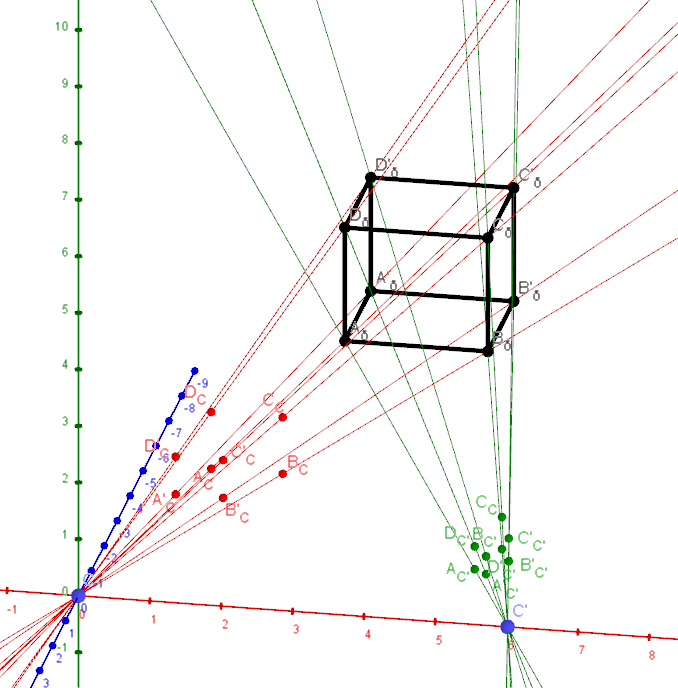
\includegraphics[width=\linewidth]{images/ScaleInvariance_1.png}
%	\caption{A really Awesome Image}
	\label{fig:awesome_image1}
	\endminipage\hfill
	\minipage{0.42\textwidth}
	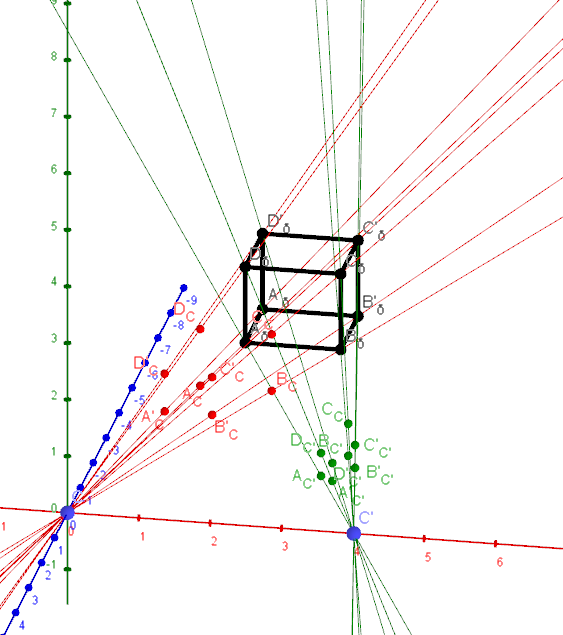
\includegraphics[width=\linewidth]{images/ScaleInvariance_2.png}
%	\caption{A really Awesome Image}
	\label{fig:awesome_image2}
	\endminipage\hfill
\end{figure}


\begin{minipage}{\linewidth}
	\centering
	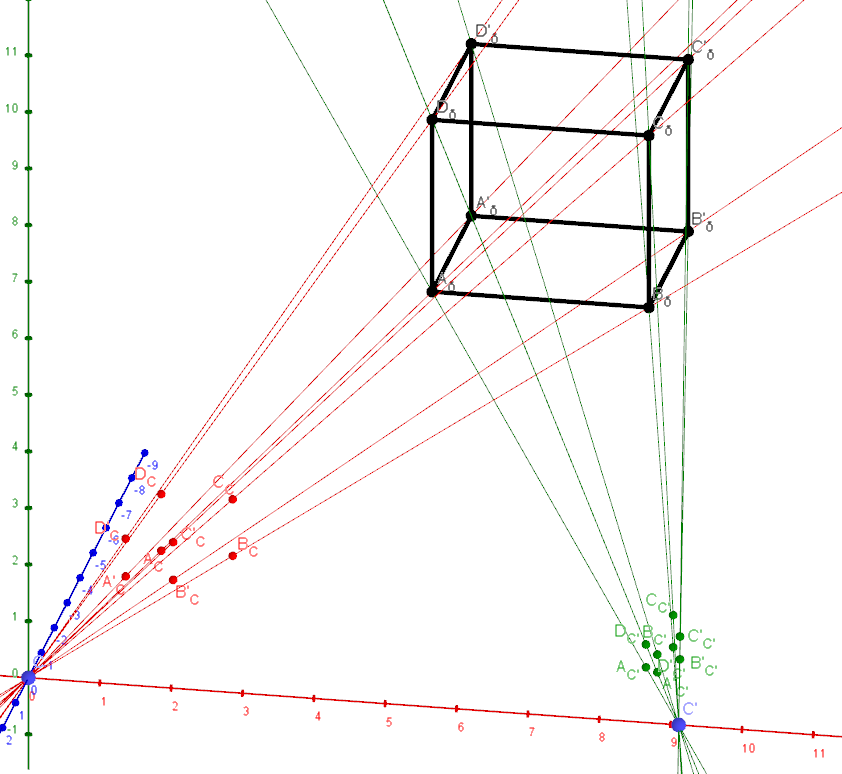
\includegraphics[width=0.42\linewidth]{images/ScaleInvariance_3.png}
	\captionof{figure}{Veranschaulichung der Skaleninvarianz und dessen Auswirkung auf die geometrische Form der Objekte} 
\end{minipage}\\ \\

\begin{figure}[!htb]
	\minipage{0.42\textwidth}
	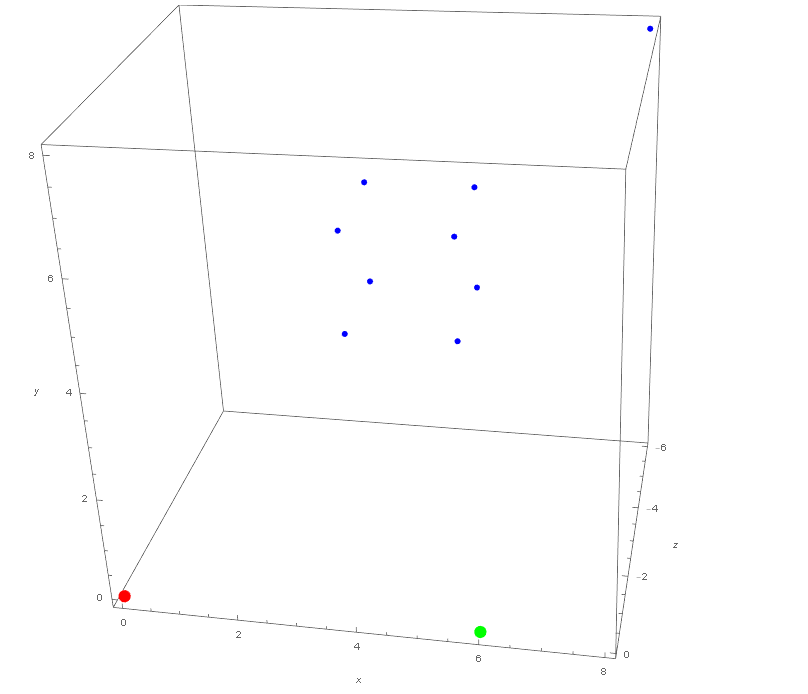
\includegraphics[width=\linewidth]{images/MinimalBeispiel_reconstructed.png}
	%	\caption{A really Awesome Image}
	\label{fig:awesome_image1}
	\endminipage\hfill
	\minipage{0.42\textwidth}
	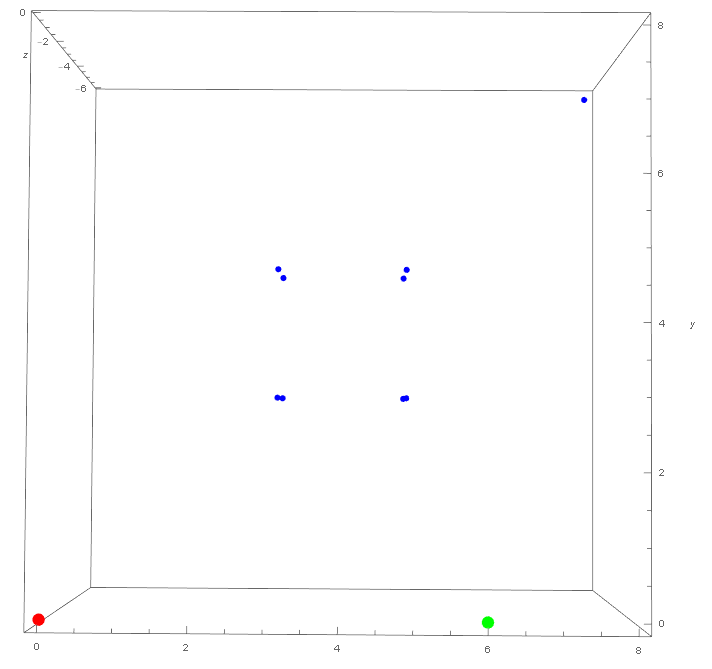
\includegraphics[width=\linewidth]{images/MinimalBeispiel_reconstructed_3.png}
	%	\caption{A really Awesome Image}
	\label{fig:awesome_image2}
	\endminipage\hfill
	\captionof{figure}{auf Originalgröße skalierte rekonstruierte Szene}
\end{figure}

\pagebreak
Abbildung 4.7 zeigt die Komplett rekonstruierte Szene des Minimalbeipiels, welche beweist, dass die beschriebenen Methoden für das Minimalbeispiel mit reinen Daten und auch bei Kameras mit unterschiedlichen Auflösungen, funktioniert hat. 

\section{Rektifizierung}
\label{sec:rectification}


%Such a pencil of lines may be considered as a 1-dimensional projective
%space. It is clear from figure 9.6b that corresponding epipolar lines are perspectively
%related, so that there is a homography between the pencil of epipolar lines centred at e
%in the first view, and the pencil centred at e in the second.\cite{HZ}


Im Minimalbeispiel ist die Triangulierung und Rekonstruktion der 3D-Weltpunkte ohne Kommunikationen durchführbar. Das liegt daran, dass mit reinen Werten gerechnet wird und Fehler wie Beispielsweise Bildrauschen nicht vorkommen. Im Minimalbeispiel kann davon ausgegangen werden ,dass die Linien zweier korrespondierender Punkte sich, welche durch die jeweilien Kamerazentren und Bildpunkte gehen, sich ziemlich sicher in einem Punkt treffen werden. In einem Beispiel mit realen Daten ist es nicht unwahrscheinlich, dass die herausgefilterten korrespondierenden Punkte, nicht zu hundert Prozent stimmen. Es kommt immer zu kleineren Abweichungen, was dazu führen kann, dass wenn die Linien der korrespondierenden Punkte im Realbild sich nicht treffen. Ein Grund dafür ist, dass sie nicht hundertprozentig auf der selben Höhe im Bild liegen und die Linien sich somit verfehlen\\



 (BILD EINFÜGEN. weiß noch nicht genau wie das aussehen soll....).\\




 Im Realbeispiel dieser Arbeit wird das Auftreten solcher Fehler durch das sogenannte \textit{Sampson-Approximation} - Verfahren behoben, welches bei kalibrierten Fällen zum einsatz kommt\cite{HZ}. Mehr zu diesem Verfahren wird im Kapitel \nameref{sec:sampson} aufgeführt. Das ist eine Möglichkeit um eine Szenerekonstruktion trotz Fehlerhafter korrespondierender Punkte zu ermöglichen. Ein weiteres weit verbreitetes Verfahren, ist cor der Szenenrekonstruierung durch Triangulierung eine Rektifizierung beider Bilder vorzunehmen\cite{MatlabRec,ZZ,Javier,Fusiello}. Da bestimmte Formen der Rektifizierung keine vorherige Kalibrierung der Kameras benötigen, wird diese Methode in den meisten gängigen Echtzeit-Szenenrekonstruktionen eingesetzt. \cite{Fusiello,Javier,R.H.}.
 Rektifizierte Bilder müssen zwei Eigenschaften erfüllen. Zum einen müssen alle Epipolargeraden parallel zur x-Koordinatenachse verlaufen und zweitens müssen alle korrespondierenden Punkte die selben y-Koordinaten besitzen\cite{ZZ}. Mit Hilfe dieser Eigenschaften ist es somit möglich die enstandenen korresponierenden Epipolarlinien als horizontale Scanlinien zu benutzen\cite{Javier,ZZ}. Mit hilfe dieser Scanlinien und den darauf sich befindenden korrespondierenden Punkte ist es zum Beispiel Möglich eine Tiefenkarte des Bildes zu berechnen allein durch die Differenz der horizontalen Lage der korrespondierenden Punkte\cite{Javier,ZZ}. \\
 
 
 \begin{minipage}{\linewidth}
 	\centering
 	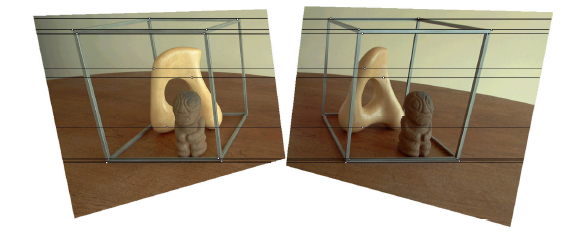
\includegraphics[width=1.\linewidth]{images/rectifiziertesBildAusZZ.png}
 	\captionof{figure}{Beipiel eines rektifizierten Bildes. Quelle: \cite{ZZ}} 
 \end{minipage}\\ \\

 \begin{minipage}{\linewidth}
	\centering
	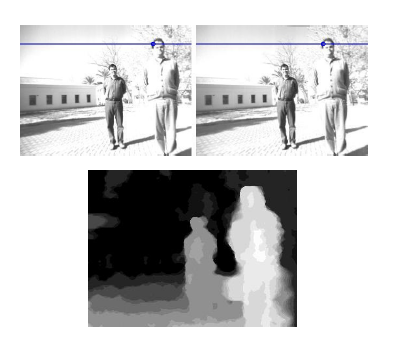
\includegraphics[width=1.\linewidth]{images/Disparity.png}
	\captionof{figure}{Beispiel einer einfachen Tiefenkarte eines Stereobildpaares nach der Rektifizierung. Quelle: \cite{Javier}} 
\end{minipage}\\ \\
 
Die Rektifizierung, allem voraus vor allem die Optimierung des Rektifizierungvorgangs, von Stereo- oder auch mulitplen- Kamerasystemen, wird heutzutage von vielen Entwicklergruppen der Computer Vision untersucht(Der satz ist mist!). Es gibt mittlerweile viele Ansätze, jedoch funktionieren nicht alle bei den selben Fällen. So setzten zum Beispiel manche Rektifizerungsalgorithmen voraus, dass die Bilder von Kameras mit selber Auflösung aufgenommen wurden. Ein Beispiel ist die Rektifizierung welche in \textit{Matlab} verwendet wird \cite{MatlabRec}. Die Rektifizierung wurde anhand einer Methode implementiert, welcher sich ähnlich verhält wie in \cite{FusielloSite} beschrieben. Die Grundidee hier hinter ist, dass die Kameramatrizen von zwei Kameras so aufgebaut sind dass die intrinsischen Parameter die selben sind, sie sich aber in ihren Rotationen und Translationen voneinander unterscheiden. Die extrinsischen Kameraparameter werden dann dementsprechend so manipuliert, dass die Bildebenen Achsenparallel zueinander stehen\cite{FusielloSite,Fusiello}. Um horizontale Epipolarlinien zu erhalten muss gleichzeitig die Basislinie zwischen den zwei Kamerazentren parallel zur neuen x-Achse beider Kameras sein. Zudem soll, um eine angemessene Rektifizierung zu gewährleisten, müssen konjugierende Punkte die selbe vertikale Koordinate haben. Dies wird hier durch die die Bedingung gewährleistet, dass beide Kameras die selben intrinsischen Parameter haben\cite{FusielloSite}. Eine Frage welche mit unter in dieser Arbeit beantwortet werden sollte, war, ob es möglich ist, ohne deutlich größeren Aufwand eine Kamerakalibrierung und Szenerekonstruktion mit Kameras unterschiedlicher Auflösung zu gewährleisten. Im Kapitel \nameref{sec:epipolar}, in welchem ausführlich die Epipolargeometrie vorgestellt wurde, wurde bereits bezug auf die unterschiedlichen Auflösungen genommen. Prinzipiell spielen unterschiedliche intrinsische Kameraparameter keine Rolle, wenn es um die Rekonstruktion der Kameraposen geht, da die Fundamental Matrix und die essentielle Matrix die Information über die intrinsischen und extrinsischen Kameraparameter besitzen und es klar gestellt wurde, dass die Bildkoordinatensysteme der Kameras nicht identisch sein müssen. \cite{Elements}. In dieser Arbeit wurde ein Rektifizierungsalgorithmus nach \textit{Zhang}\cite{ZZ} implementiert, welcher sich die Fundamentalmatrix zu nutzen macht. \textit{Loop} und \textit{Zhang} zerlegen jede Kollinearität in eine Ähnlichkeitstransformation, eine Schertransformation und eine projektive Transformation. Die projektive Komponenten wird dabei in einem nichtlinearen Optimierungsprozess so affin wie möglich gemacht.\cite{Fusiello,ZZ}. Im folgenden wird zunächst der genaue Vorgang des implementierten Algorithmus genauer erklärt und 
\textcolor{red}{des Weiteren werden zwei Beispiele vorgestellt, welche die Bilder des Minimalbeispiels einmal mit gleichen intrinsischen Parametern und einmal mit unterschiedlichen intrinsischen Parametern der Kamera aufzeigt. Es wird sich Herausstellen, dass beide Beispiele eine gelungene Rektifizierung der Bilder aufweisen.(Nochmal genau nachprüfen ob das geht!!!)}. Während sich einige Rektifizierungsverfahren im 3D-Raum abspielen, wird beim Verfahren nach \textit{Zhang}, hauptsächlich im 2D-Raum gearbeitet. Des Weiteren wird vorausgesetzt, dass die Fundamental Matrix \textit{F} und somot auch korrespondierende Punkte bereits bekannt sind. Sind die intrinsischen Kameraparameter bekannt, so wird aus der Fundamentalmatrix die Essentielle Matrix. Das Verfahren kann sowohl in einem kalibrierten als auch in einen unkalibrierten Fall angewendet werden\cite{ZZ}. Im Algorithmus wurde der unkalibrierte Fall implementiert und somit wird in der Erläuterung und in den danach folgenden Beispielen die Fundamentalmatrix \textit{F} verwendet. Die korrespondierenden Punkte werden mit \textit{x} für das erste beziehungsweise \textit{x'} für das zweite Bild definiert, die Kamerazentren dementsprechend mit \textit{C} und \textit{C'}. Bildebene der ersten Kamera wird mit \textit{I} definiert und die Bildebene von Kamera zwei mit \textit{I'}, die entsprechenden Epipole mit \textit{e} und \textit{e'}. Der Prozess der im Algorithmus erfolgt kann quasi als eine Transformation der Epipolar Geometrie eines Bildpaares in eine kanonische Form angesehen werden. Diese Transformation wird durch eine Homographiematrix durchgeführt, welche sich aus den bereits erwähnten drei Komponenten zusammenstellt. Zu Beginn sei noch erwähnt dass wir pro Bild zwei unterschiedliche Homographien \ensuremath{H} und \ensuremath{H'} brauchen. Die Fundamentalmatrix liefert, die Epipolarbedingung, dass $x'^TFx=0$ ergibt, wenn $x'$ auf der zu $x$ korrespondierenden Epipolarlinie liegt. Die korrespondierenden Punkte $x$ und $x'$ werden, für die Rektifizierung, jeweils mit den Homographien $H$ und $H'$ verrechnet.

\begin{gather}
	\bar{x}= Hx\\
	\bar{x'}= Hx'
\end{gather}\\

Die Fundamentalmatrix, welche sich aus durch die Rektifizierten korrespondierenden Punkte resultiert, wird mit $\bar{F}$ bezeichnet. Daraus folgt für die Fundamentalmatrix folgendes:

\begin{gather}
	\bar{x'}^T\bar{F}\bar{x} = 0\\
	\leadsto x'^TH'T\bar{F}Hx=0\\
	\leadsto F = H'^T[i]_xH
\end{gather}\\

Das Ziel ist es diese zwei Homographien in deren bereits erwähnten projektiven und affinen Komponenten zu zersetzten, wobei diese die jeweils entstehenden Bildverzerrungen minimieren sollen. Die Homographiematrizen bestehen aus drei Linien, welche jeweils durch den Epipol verlaufen. Des Weiteren werden noch ein paar weitere Bedingungen für die jeweils drei Linien festgelegt. So müssen die Linien $v$ und $v'$ sowie $w$ und $w'$ korrespondierende Epipolarlinien sein. Diese Bedingung schafft eine geometrische Verbindung beider Bilder zueinander und ist gerade bei der Minimierung der durch die Rektifizierung entstehenden Bildverzerrung von Bedeutung.

\begin{gather}
H = \begin{bmatrix}
u^T\\v^T\\w^T
\end{bmatrix} =
\begin{bmatrix}
u_a&u_b&u_c\\
v_a&v_b&v_c\\
w_a&w_b&w_c
\end{bmatrix}\\
H' = \begin{bmatrix}
u'^T\\v'^T\\w'^T
\end{bmatrix} =
\begin{bmatrix}
u'_a&u'_b&u'_c\\
v'_a&v'_b&v'_c\\
w'_a&w'_b&w'_c
\end{bmatrix}	
\end{gather}\\

Für die Bestimmung der einzelnen Komponenten von $H$ und $H'$ werden diese in ihre projektiven und affinen Teilstücke zerlegt. Davor wird noch die letzte Komponente $w_c$ raus dividiert, um somit  skaleninvariante Matrizen $H$ und $H'$ zu bekommen. 

\begin{gather}
H = \begin{bmatrix}
u^T\\v^T\\w^T
\end{bmatrix} =
\begin{bmatrix}
u_a&u_b&u_c\\
v_a&v_b&v_c\\
w_a&w_b&1
\end{bmatrix}\\
H' = \begin{bmatrix}
u'^T\\v'^T\\w'^T
\end{bmatrix} =
\begin{bmatrix}
u'_a&u'_b&u'_c\\
v'_a&v'_b&v'_c\\
w'_a&w'_b&1
\end{bmatrix}	
\end{gather}\\

Beide Matrizen werden nun auf die selbe Weise in ihre projektiven und affinen Bestandteile zerlegt.

\begin{gather}
	H = H_p \cdot H_a\\
	H' = H'_p \cdot H'_a
\end{gather}\\

$H_p$ ist die projektive Komponente, sie bezieht sich nur auf die letzte Zeile der Matrix $H$ und wirkt sich somit auch nur auf die homogene Komponenten der mit ihr verrechneten Punkte aus. 

\begin{gather}
	H_p = 
	\begin{bmatrix}
		1&0&0\\
		0&0&1\\
		w_a&w_b&1
	\end{bmatrix}
\end{gather}\\

Die affine Komponeten $H_a$ lässt sich aus $H$ und $H_p$ konstruieren. Es gilt:

\begin{gather}
	H_a= H \cdot H^{-1}_p = 
	\begin{bmatrix}
	u_a-v_cw_b&v_cw_a-v_a&0\\
	v_a-v_cw_a&v_b-v_cw_b&v_c\\
	0&0&1
	\end{bmatrix}
\end{gather}

Für die Matrizen $H_p'$ und $H_a'$ gilt das selbe nur mit den Epipolarlinien $u'$, $v'$ und $w'$.
Die projektive Matrix sogt dafür, dass die Epipole beider Bilder ins unendliche gesetzt werden und die Epipolarlinien der Bilder jeweils parallel zueinander verlaufen. Zu Beginn wurde erwähnt dass es eine Zerlegung in eine projektive, eine Ähnlichkeits- und eine Scherungstransformation gibt. Die projektive Komponente ist mit $H_p$ und $H_p'$ bereits vollständig definiert. Was nun noch fehlt ist die Zerlegung der affinen Matrizen $H_a$ und $H_a'$ in ihre jeweiligen Ähnlichkeits- und Scherungstransformationen. 

\begin{gather}
	H_a = H_s \cdot H_r\\
	H_r = 
	\begin{bmatrix}
	v_b-v_cw_b&	v_a-v_cw_a&0\\
	v_a-v_cw_a&v_b-v_cw_b&v_c\\
	0&0&1
	\end{bmatrix}\\
	H_s = 
	\begin{bmatrix}
	u_a&u_b&u_c\\
	0&1&0\\
	0&0&1
	\end{bmatrix}
\end{gather}\\

$H_r$ und auch $H_r'$ definieren eine Rotation und auch eine Verschiebung, welche die bereits parallelen Epipolarlinien beider Bilder zueinander parallel und horizontal ausrichtet. Durch die Verschiebung werden die korrespondierenden Epipolarlinien noch auf die selbe Höhe verschoben. Somit entstehen die gewünschten Scanlinien in den Bildern. Die Matrix $H_s$ und $H_s'$ wirken sich nur auf die $u$-Elemente der Matrix $H$ und $H'$ aus und definieren eine Scherung. Sie haben keine Auswirkung auf die Rektifizierung an sich aber sorgen dafür, dass die horizontale Verzerrung der beiden Bilder zueinander reduziert wird.\\

\subsection{Projektive Transformation}

Die projektiven Matrizen $H_p$ und $H_p'$ werden von den Linien $w$ und $w'$ bestimmt. $w$ und $w'$ sind dabei jedoch nicht unabhängig. Definiert werden sie durch einen Punkt $z = \begin{bmatrix}
\lambda&\mu&0\end{bmatrix}^T$, welche die, durch die Rektifizierung entstehende, Bildverzerrung minimieren soll. Für beide Bilder werden $w$ und $w'$ folgendermaßen gewählt

\begin{gather}
	w = [e]_x \cdot z\\
	w'= F\cdot z
\end{gather}\\

Jedes beliebige $z$ würde zwei korrespondierende Epipolarlinien definieren, um ein $z$ zu finden, welches die Verzerrung der Bilder minimiert, wird ein Kriterium aufgestellt, welches ein $z$ finden soll, dass die Verzerrung minimal halten wird. Minimierung bedeutet in diesem Falle, dass versucht wird die Matrizen $H_p$ und $H_p'$ so affin wie möglich zu machen. So affin wie möglich bedeute, dass die Werte von $w_a$ und $w_b$ so nah wie möglich an den Wert 0 gebracht werden sollen.

\begin{gather}
	H_p = 	\begin{bmatrix}
	1&0&0\\
	0&0&1\\
	w_a&w_b&1
	\end{bmatrix}
\end{gather}

Jedoch sollen sie nicht ganz null werden, da die projektive Matrix dann keine projektive mehr wäre, sondern eine affine.  Deswegen heißt es auch sie soll so affin wie möglich gemacht werden. Das selbe gilt natürlich auch für $w_a'$ und $w_b'$ aus $H_p'$. Wäre das der Fall, so wären die beiden Epipole $e$ und $e'$ bereits im unendlichen und die Matrizen $H_p$ und $H_p'$ hätten keine Auswirkungen auf die Punkte. Für die Minimierung wird die Methode des \textit{least-square-fitting}, also die Anpassung des kleinsten Quadrats, genutzt\cite{leastSquare}. Es werden also die Gewichtungen der Punkte in beiden Bildern in der Methode der Anpassung der kleinsten Quadrate verbaut, welche versucht eine Funktion zu finden, die einen Wert für $z$ berechnen soll welcher die Bildverzerrung minimal hält. \textcolor{red}{Anders ausgedrückt man sucht einen Wert für $z$, welcher am nächsten an den gegebenen Punktesammlungen der jeweiligen Bildern dran liegt, wobei für $z$ bereits gilt, dass es sich um einen Punkt im Unendlichen handeln soll}\cite{ZZ,leastSquare}. Angenommenem, dass die Annäherungsfunktion $g(x)$ eine Funktion $f(x)$, mit $x \in [a,b]$, annähern soll, dann versucht die Methode, die Summe der Quadrate der oridnatischen Differenzen, welche zwischen den von der Funktion generierten Punkten und den Punkten aus den Daten gewonnen wird, zu minimieren\cite{leastSquare,Margulies.}. Zum Beispiel werden $n$ Datenpunkte angenommen, dann gilt:

\begin{gather}
	e = \sum_{i=1}^{n}[f(x_i)-g(x_i)]^2
\end{gather}

Für die Minimierung der Bildverzerrung werden die Gewichtungen der Punkte beider Bilder benötigt. $p_i$ beinhaltet alle Punkte von Bild eins und $p_j$ beinhaltet alle Punkte von Bild zwei. Angenommen wir nehmen einen Punkt aus Bild eins $p_{i1} = \begin{bmatrix}p_{i1,u}&p_{i1,v}&1\end{bmatrix}^T$, so soll dieser Punkt mit der Matrix $H_p$ zu einem Punkt der Form  $p_{i1} = \begin{bmatrix}\frac{p_{i1,u}}{w_i}&\frac{p_{i1,v}}{w_i}&1\end{bmatrix}^T$ transformiert werden. $w_i$ ist die Gewichtung welche durch die Verrechnung von $w$ mit $p_i$ zustande kommt.

\begin{gather}
	w_i=w^Tp_i
\end{gather} 

Ist die Gewichtung der Punkte identisch gibt es keine projektive Verzerrung und die Homographie ist eine affine Transformation. Jedoch wenn die Epipole der Bilder ins Unendliche transformiert werden sollen, so können $H_p$ und $H_p'$ keine affine Homograhien sein. Sonst könnte man die Epipole nur innerhalb der affinen Ebenen, sprich den Bildebenen, verschieben. Also bildet der Versuch $H_p$ und $H_p'$ so affin wie möglich zu machen die Basis für die Minimierung. Im Realbeispiel werden alle Pixel des Bildes verwendet. Die Rektifizierung wurde im aufgeführten Beispiel anhand des erstellten Minimalbeispiels durchgeführt, somit wurden die Eckpunkte des Quaders des jeweiligen Bildes für die das Minimierungskriterium verwendet. Es wird eine Funktion nach dem Prinzip der Anpassung der kleinsten Quadrate aufgestellt, welche die Abweichung der Gewichtung der Punkte in Bezug auf die Gewichtung des Bildzentrums $p_c$ berechnet.$p_c$ ergibt sich aus der Mittelung aller verwendeten Punkte eines Bildes $p_c = \frac{1}{n} \sum_{i=1}^{n} p_i$, dessen Gewichtung ergibt sich aus $w_c= w^T p_c$. Die gesuchte Abweichung ausgedrückt in der Anpassung der kleinsten Quadreate ergibt dann die folgende Formel.\\

\begin{gather}
	\sum_{i-1}^{n}\Big[\frac{w_i-w_c}{w_c} \Big]^2\\
	\leadsto \sum_{i=1}^{n}\Big[\frac{w^T (p_i-p_c)}{w^Tp_c} \Big]^2
	\leadsto \sum_{i=1}^{n}\Big[\frac{w^T (p_i-p_c)(p_i-p_c)^Tw}{w^Tp_cp_c^Tw} \Big]
\end{gather}\\

Vereinfacht lässt sich das auch in einer Matrixgleichung angeben

\begin{gather}
	\frac{w^TPP^Tw}{w^Tp_cp_c^Tw}
\end{gather}

in welcher für $P$ gilt:

\begin{gather}
	P=\begin{bmatrix}
	p_{1,u}-p_{c,u}&p_{2,u}-p_{c,u}&...&p_{i,u}-p_{c,u}\\
	p_{1,v}-p_{c,v}&p_{2,v}-p_{c,v}&...&p_{i,v}-p_{c,v}\\
	0&0&...&0	
	\end{bmatrix}
\end{gather}

die Gleichungen 4.79 bis 4.83 werden ebenfalls für die Punkte $p_j$ in Bild zwei aufgestellt. So ergibt sich für das zweite Bild die Matrixgleichung:

\begin{gather}
	\frac{w'^TP'P'^Tw'}{w'^Tp_c'p_c'^Tw'}
\end{gather} 

Das Ziel ist es einen Wert für $z$ zu finden, welches bis jetzt noch nicht ersichtlich in den Gleichungen vorkommt. Also werden $w$ und $w^T$ noch mit ihren Definitionen aus den Gleichungen 4.75 und 4.76 ersetzt. Gleichzeitig werden die Gleichungen 4.82 und 4.84 summiert um die Gleichung zu erhalten, welche sich auf beide Bilder gleichzeitig bezieht und somit eine Lösung für $z$, das für beide Bilder gilt, gesucht werden kann.

\begin{gather}
	\frac{z^T[e]_x^TPP^T[e]_xz}{z^T[e]_x^Tp_cp_c^T[e]_xz}+\frac{z^TF^TP'P'^TFz}{z^TF^Tp_c'p_c'^TFz}
\end{gather}

Für den weiteren Verlauf werden die Ausdrücke noch durch die Variablen $A,B,A'$ und $B'$ vereinfacht.

\begin{gather}
	A = [e]_x^TPP^T[e]_x\\
	B=[e]_x^Tp_cp_c^T[e]_x\\
	A'=F^TP'P'^TF\\
	B'= F^Tp_c'p_c'^TF\\
	\leadsto 
	\frac{z^TAz}{z^TBz}+\frac{z^TA'z}{z^TB'Fz}
\end{gather}\\

Da die dritte Komponente von $z$ laut definition null sein soll, wird zu $z = \begin{pmatrix}
\lambda\\ \mu\end{pmatrix}$ umgeschrieben. $A,B,A'$ und $B'$ sind 3x3-Matrizen, von welchen uns dann nur noch der erste 2x2-Block interessiert. Bei dem somit aufgestellten Minimalisierungs Kriterium, handelt es sich um ein nicht lineares optimierungs Problem. Die Gleichung 4.90 ist dann minimiert, wenn die erste Ableitung dieser Funktion nach $\lambda$ = gleich null ist. Es entsteht also ein Polynom mit dem Grad sieben, da die 4.90 die Summe zweier rationaler Funktionen ist, welche jeweil das Verhältnis von quadratischen Polynomen darstellt.

\begin{gather}
\textit{Hier soll das Polynom aufgestllt werden, ist aber nicht mehr klar wie das ging!!!}
\end{gather}\\

Für die nicht lineare Optimierung wird das gesamte Polynom aufgeteilt, so minimieren wir zunächst $\frac{z^TAz}{z^TBz}$ und danach $\frac{z^TA'z}{z^TB'z}$. So entstehen für $z$ zunächst zwei Lösungen 
$\hat{z_1}$ und $\hat{z_2}$, welche über eine Mittelung eine ersten Schätzung für $z$ geben, welche schon ziemlich nah an den optimalen Wert heranreicht.

\begin{gather}
	z = \frac{\frac{\hat{z_1}}{\| z_1 \|}+\frac{\hat{z_2}}{\| z_2 \|}}{2}
\end{gather}\\

Da es sich um eine nicht lineare Optimierung handelt ist die Minimierung von  $\frac{z^TAz}{z^TBz}$ gleichzusetzen mit der Maximierung von  $\frac{z^TBz}{z^TAz}$. Beide als eine Funktion von $f(z)$. Matrix $A$ wird mit der Choleskyzerlegung in zwei höhere Dreiecksmatrizen zerlegt $A = D^TD$\cite{Fortran77}. Dies geht nur da $A$ nachweislich eine symmetrische und positiv-definite Matrix ist.\cite{Fortran77} positiv-Definite bedeutet, dass die Singulärwerte von $A$ immer positiv bleiben, egal mit welchem Vektor $z$ diese multipliziert wird. \textcolor{red}{(HIER NOCH LITERATUR FINDEN UND NOCHMAL PRÜFEN OB DEFINITION SO STIMMT)}.  Des Weiteren wir definiert, dass $y = Dz$ ist und $f(z)$ wird dann zu einen $\hat{f}(y)$

\begin{gather}
	A = D^TD\\
	y= Dz \leadsto z= D^{-1}y\\
	f(z)= \frac{z^TBz}{z^TAz}\\
	\leadsto 
	f(z)=\frac{z^TBz}{z^TD^TDz}\\
	\hat{f}(y)= \frac{y^TD^{-T}BD^{-1}y}{y^Ty}
\end{gather}

Durch die Defintion von $y = Dz$ ist $y$ bis auf einen Skalierungsfaktor definiert. $\hat{f}(y)$ ist maximiert, wenn $y$ gleich dem Eigenvektor von $D^-TBD-1$ ist, welcher mit dem größten Eigenwert assoziert wird. Zum Schluss erhalten wir dann einen Wert für $\hat{z_1}$ mit $\hat{z_1} = D^{-1}y$. Exakt das selbe Verfahren wird für die Findung von $z_2$ mit  $\frac{z^TB'z}{z^TA'z}$ angewandt. \textcolor{red}{Sind $z_1, z_2$ und eine erste Schätzung für $z$ gefunden, so kann ein Wert für $z$ gesucht werden, welcher noch näher an ein optimales Ergebnis heranreicht. Beide Lösungen $z_1$ und $z_2$, werden in die Funktion $f(z)$ eingesetzt und es jeweils ein wert ermittelt, welcher am nächsten an einem Nullpunkt sich befindet. So kann iterativ eine optimale Lösung für $z$ gefunden werden.} Ist der Wert für $z$ bestimmt, so kann dieser die Gleichungen 4.75 und 4.76 eingesetzt werden und $w$ beziehungsweise $w'$ bestimmt werden, welche die Elemente für die Matritzen $H_p$ und $H_p'$ bereitstellen.
Abbildung 4.7 zeigt in rot den Quader des Minimalbeispiels wie er in Kamera zwei abgebildet ist und in grün wie er in Kamera eins abgebildet ist. Kamera zwei ist horizontal zu Kamera eins verschoben und um $45\circ$ zu Kamera eins um die eigene vertikale Achse ein gedreht. Die Auflösungen beider Kameras sind identisch, sprich die intrinsischen Kameraparameter sind die selben. Abbildung 4.8 zeigt die momentanen Epipolarlinien. Die Epipolarlinien von Bild eins, also dem grünen Abbild, sind bereits Parallel, was aber keine Voraussetzung für die Funktion des Rektifizierungsalgorithmus ist. Der Schnittpunkt der Epipolarlinien von Bild zwei, also dem Roten Abbild, treffen sich in einem Punkt und bilden somit den Epipol von Bild zwei. 

\begin{minipage}{\linewidth}
	\centering
	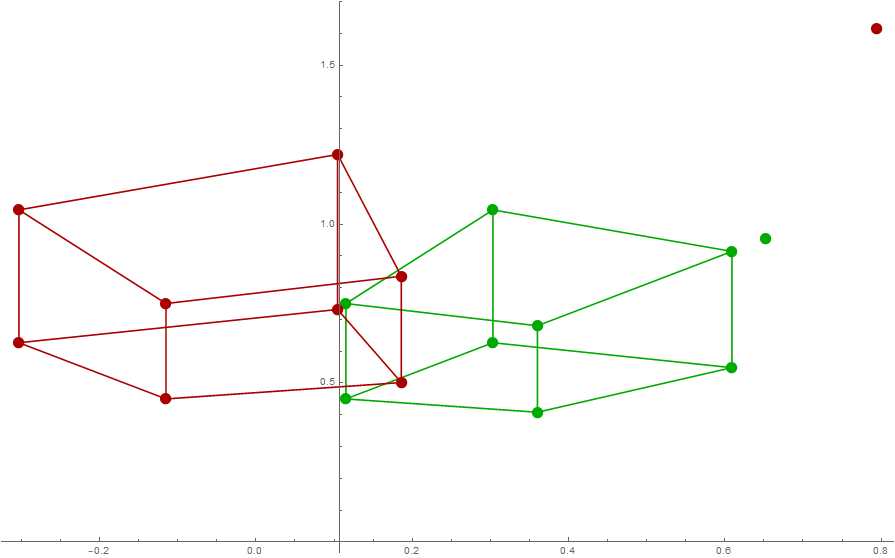
\includegraphics[width=.8\linewidth]{images/Rectification_one_same_Solutions.png}
	\captionof{figure}{Aufnahmen zweier Kameras mit den selben Auflösungen, Kamera eins(Grün) und Kamera(rot) zwei gelten jeweils \ensuremath{\zeta =1}} 
\end{minipage}\\ 

\begin{minipage}{\linewidth}
	\centering
	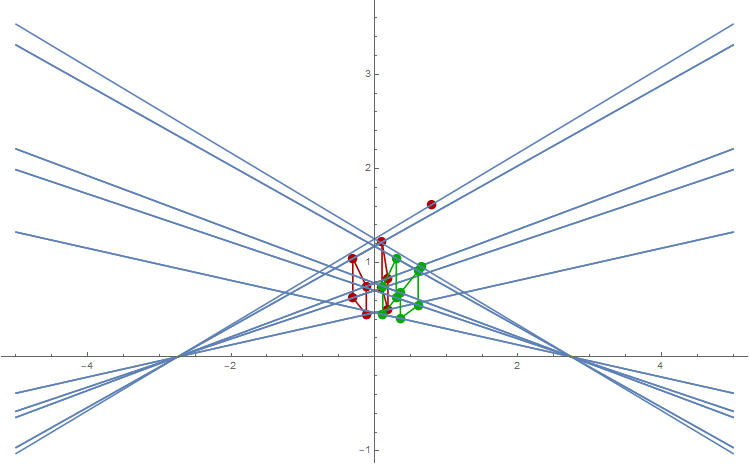
\includegraphics[width=.8\linewidth]{images/Rectification_two_same_Solutions.png}
	\captionof{figure}{Epipole für Kamera eins und Kamera zwei vor der Rektifizierung } 
\end{minipage}\\


Werden nun die Matritzen $H_p$ und $H_p'$ auf die jeweiligen Punkte der Bilder, $p_i$ für Bild eins und $p_j$ für Bild zwei, angewandt, so kann man eine erste Veränderung beobachten. Abbildung 4.9 zeigt beide Quader aus Abbildung 4.7 nachdem die jeweiligen Bildpunkte mit den projektiven Matrizen multipliziert wurden. Der Epipol in Bild eins bleibt natürlich wie zuvor im unendlichen, jedoch kann man erkennen, dass der rote Quader aus Bild zwei sich verändert hat. Sein Epipol wurde ins Unendliche transformiert und parallele Linien sind nun auch auf dem Bild parallel. Das die Epipolarlinien bereits horizontal parallel zur x-Achse verlaufen ist Zufall und ist nach der Anwendung der projektiven Matrizen auch noch nicht verlangt. Das Anpassen der Epipolarlinien, dazu gehört sie zunächst von beiden Bilder aus parallel zur x-Achse verlaufen zu lassen und dann noch sie so zueinander anzupassen, dass sie zu Scanlinien über beide Bilder verlaufen, verlgeiche Abbildung 4.12, folgt im nächsten Schritt. \\


\begin{minipage}{\linewidth}
	\centering
	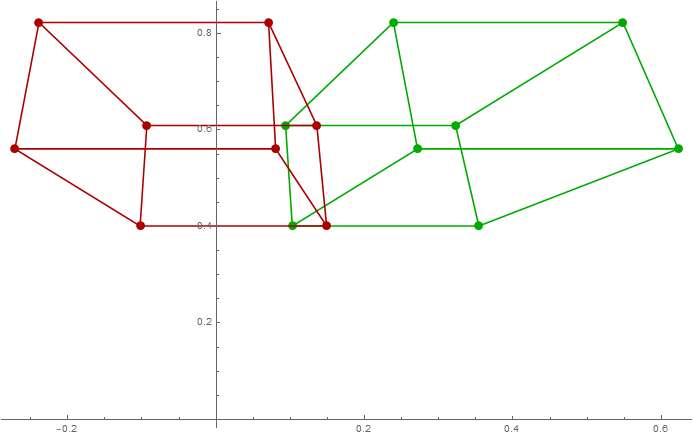
\includegraphics[width=1.\linewidth]{images/Rectification_Hp_same_Solutions.png}
	\captionof{figure}{Abbildung beider Bilder nach anwenden der Matrizen $H_p$ und $H_p'$. Die Epipole beider Bilder sind nun im unendlichen. Das die enstehenden parallelen Epipolarlinien auch hier schon horizontal ausgerichtet sind ist Zufall. Die Epipolarlinien sind immer parallel nach dieser Transformation aber die Richtung ist nicht immer automatisch bereits i = [1,0,0].} 
\end{minipage}\\ \\

\subsection{Ähnlichkeitstransformation}

Nachdem die Epipole ins Unendliche verschoben wurden, müssen diese nun so rotiert und verschoben werden, dass die Epipolarlinien als Richtung $i = \begin{bmatrix}1&0&0\end{bmatrix}$ haben und die Epipolarlinien beider Bilder zu einheitlichen Scanlinien werden. Für die Ähnlichkeitstransformation wird davon ausgegangen, dass $w$ und $w'$ bereits bekannt sind.$H_r$ und $H_r'$ wurden bereits aus der Zerlegung von $H_a$ und $H_a'$ gewonnen.

\begin{gather}
		H_r = 
	\begin{bmatrix}
	v_b-v_cw_b&	v_a-v_cw_a&0\\
	v_a-v_cw_a&v_b-v_cw_b&v_c\\
	0&0&1
	\end{bmatrix}\\
		H_r' = 
	\begin{bmatrix}
	v_b'-v_c'w_b'&	v_a'-v_c'w_a'&0\\
	v_a'-v_c'w_a'&v_b'-v_c'w_b'&v_c'\\
	0&0&1
	\end{bmatrix}\\
\end{gather}

$w$ und $w'$ sind bereits bekannt, Mit Hilfe von $F$, können $v_a$ und $v_b$ ersetzt werden. Dazu kann die letzte Zeile von F nach $v_a, v_b$ und $v_c$ aufgelöst werden. Für $v_a', v_b'$ und $v_c'$ wird die letzte Spalte von F verwendet. So können folgende Gleichungen für $v_a, v_a',v_b, v_b', v_c$ und $v_c'$ gewonnen werden. 

\begin{gather}
	F = H'^T[i]_xH\\
	F=
	\begin{bmatrix}
	v_aw_a' - v_a'w_a&v_bw_a' - v_a'w_b&v_cw_a' - v_a'\\
	v_aw_b' - v_b'w_a&v_bw_b' - v_b'w_b&v_cw_b' - v_b'\\
	v_a - v_c'w_a&v_b - v_c'w_b&v_c-v_c'
	\end{bmatrix}\\
	v_a = F_{31}+v_c'w_a\\
	v_b = F_{32}+v_c'w_b\\
	v_c = F_{33}+v_c'\\
	v_a' = v_cw_a'-F_{13}\\
	v_b' = v_cw_b'-F_{23}\\
	v_c' = v_c -F_{33}
\end{gather}

Eingesetzt in die jeweiligen Matrizen $H_r$ und $H_r'$, entstehen die folgenden Matrizen in Gleichungen 4.114 und 4.115, welche nur noch die unbekannte $v_c'$ beinhalten. Die gemeinsame Variable $v_c'$ zeigt die geometrische Verbindung beider Bilder in ihrer Verschiebung entlang ihrer v-Richtung. Es wird also ein Offset von $F_33$ benötigt, um die Epipolarlinien horizontal zu Scanlinien auszurichten. \textcolor{red}{Den Wert für $v_c$ wird so ermittelt, dass das Minimum einer v-Koordinaten eines Pixel als minimum den Wert null besitzt }

\begin{gather}
	H_r = \begin{bmatrix}
	F_{32}-w_bF_{33}&w_aF_{33}-F_{31}&0\\
	F_{31}-w_aF_{33}&F_{32}-w_bF_{33}&F_{33}+v_c'\\
	0&0&1
	\end{bmatrix}\\
	H_r'=
	\begin{bmatrix}
	w_b'F_{33}-F_{23}&F_{13}-w_a'F_{33}&0\\
	w_a'F_{33}-F_{13}&w_b'F_{33}-F_{23}&v_c'\\
	0&0&1
	\end{bmatrix}
\end{gather}\\

Das Ergebnis der Bildpunkte $p_i$ und $p_j$ multipliziert mit den Matrizen $H_rH_p$ und $H_r'H_p'$ mit ist in Abbildung 4.10 zu sehen. Als letztes folgt noch die Scherungstransformation $H_s$ und $H_s'$ für die horizontale Entzerrung beider Bilder.\\ 

\begin{minipage}{\linewidth}
	\centering
	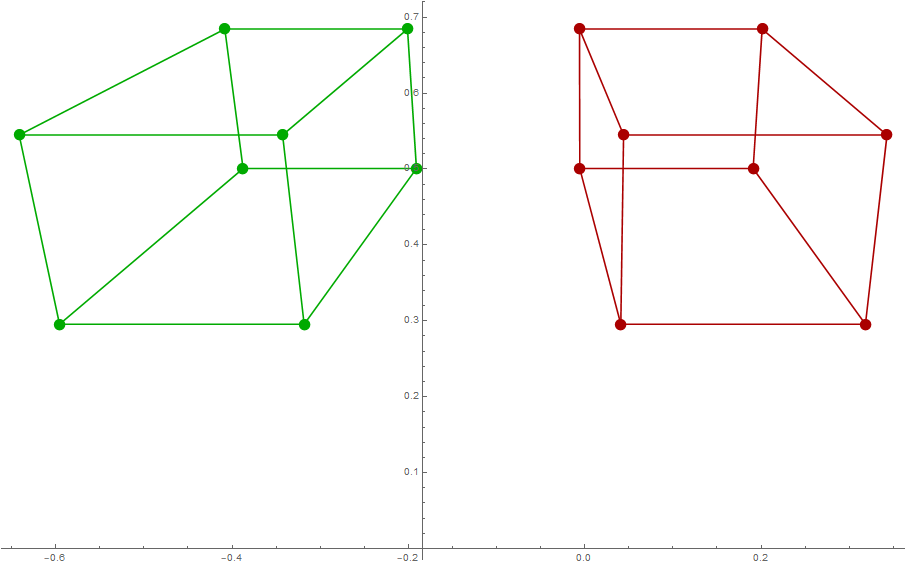
\includegraphics[width=1.\linewidth]{images/Rectification_HrHp_same_Solutions.png}
	\captionof{figure}{Abbildung beider Bilder nach anwenden der Matrizen $H_r \cdot H_p$ und $H_r' \cdot H_p'$. Die Epipolarlinien sind nun horizontal zueinander ausgerichtet} 
\end{minipage}\\ \\

\subsection{Scherungstransformation}

Die letzte Transformation, welche an den Bilder durchgeführt werden soll, ist die sogenannten Scherungstransformation. Sie soll vor allem dazu dienen, die horizontale Verzerrung der Bilder zueinander nochmal weiter zu minimieren. Die Matrizen $H_s$ und $H'_r$ wirken sich hauptsächlich auf die $u$ und $u'$ Komponenten aus. 

\begin{gather}
	H_s =\begin{bmatrix}
	u_a&u_b&0\\
	0&1&0\\
	0&0&1
	\end{bmatrix}\\
		H'_s =\begin{bmatrix}
	u'_a&u'_b&0\\
	0&1&0\\
	0&0&1
	\end{bmatrix}
\end{gather}

Um die richtigen Werte für $a, a', b$ und $b'$ zu bekommen, werden zunächst Punkte an den jeweiligen gegenüberliegenden Kanten der Bilder definiert. Da die Bilder des Quaders nicht aus tausenden von Pixeln bestehen, wie ein reales Bild, sondern nur über dessen Eckpunkte bestimmt ist, wird eine Bildbreite $w$ und $w'$ und eine Bildhöhe $h$ und $h'$ definiert. Die Höhen und Breiten der Bilder rahmen die abgebildeten Quader ein, somit wurde quasi eine Bildgröße für beide Bilder definiert. Nun können die Punkte an den Kantenhalbierenden $a = [\frac{w-1}{2} \; 0 \; 1]^T, b = [w-1 \; \frac{h-1}{2}\; 1]^T, c = [\frac{w-1}{2} \; h-1 \; 1]^T, d = [0 \; \frac{h-1}{2} \; 1]^T$ gebildet werden. Der Gedanke, der damit verfolgt wird ist, dass die Punkte der jeweiligen gegenüberliegenden Kanten mit einander verbunden werden können und dann so ausgerichtet werden sollen, dass sie sich wieder direkt gegenüber liegen. Schematisch wird as in Abbildung ???? aufgezeigt.

\begin{minipage}{\linewidth}
	\centering
	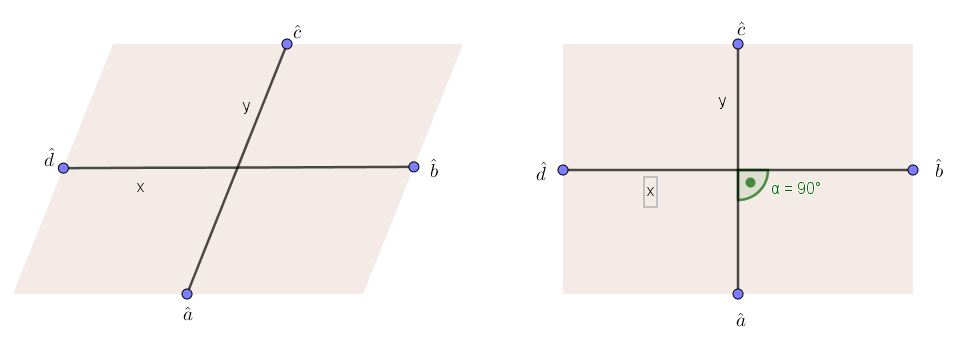
\includegraphics[width=.8\linewidth]{images/Scherungstransformation.png}
	\captionof{figure}{Die Abbildung verdeutlicht noch mal Schematisch, wie sich die Punkte ausrichten sollen. Bild a) zeigt die durch die Rektifizierung verschobenen Bildkantenmitten. Bild b= zeigt, wie sich die Bildkantenmitten durch die Scherungstransformation wieder ausrichten sollen.} 
\end{minipage}\\ \\

Die Punkte $a,b,c,d$ und auch $a',b',c',d'$ geben die Bildbreiten der noch unberührten Bilder an. Nach der Rektifizierung sind die Bilder so verzerrt, dass die Kanten mitten sich meistens nicht mehr direkt gegenüber von einander befinden. Die Punkte $a,b,c,d$ und $a',b',c',d'$ werden mit den Matrizen $H_p, H'_p, H_r$ und $H'_r$ verrechnet, so dass man die genaue neue Position der Kanten Mitten nach der Rektifizierung hat. 

\begin{gather*}
	\hat{a} = H_r\cdot H_p \cdot a\\
	\hat{b} = H_r\cdot H_p \cdot b\\
	\hat{c} = H_r\cdot H_p \cdot c\\
	\hat{d} = H_r\cdot H_p \cdot d\\
	\hat{a'} = H'_r\cdot H'_p \cdot a'\\
	\hat{b'} = H'_r\cdot H'_p \cdot b'\\
	\hat{c'} = H'_r\cdot H'_p \cdot c'\\
	\hat{d'} = H'_r\cdot H'_p \cdot d'\\
\end{gather*}

Um aus $\hat{a},\hat{b},\hat{c},\hat{d}$ und auch $\hat{a}',\hat{b}',\hat{c}',\hat{d}'$ wieder Punkte der affinen Ebene zu machen werden sie jeweils durch ihre dritte Komponenten geteilt, so das $\hat{a}_w,\hat{b}_w,\hat{c}_w,\hat{d}_w$ und $\hat{a}'_w,\hat{b}'_w,\hat{c}'_w,\hat{d}'_w$ jeweils den Wert eins besitzen. Danach können die Vektoren $\vec{x}$ und $\vec{y}$ aus den Differenzen der sich ursprünglich gegenüberliegenden Punkte gebildet werden.

\begin{gather}
	x = \hat{b}-\hat{d}\\
	y = \hat{c}-\hat{a}\\
	x' = \hat{b}'-\hat{d}'\\
	y' = \hat{c}'-\hat{a}'
\end{gather}

$x$ und $y$ sind Vektoren der euklidischen Bildebene. Die Rechwinkligkeit beider wird also erhalten, wenn gilt:

\begin{gather}
	(H_sx)^T(H_sy)= 0 \\
	(H'_sx')^T(H'_sy')= 0 
\end{gather}

Die Seitenverhältnisse der Bilder werden beibehalten, wenn gilt:

\begin{gather}
	\frac{(H_sx)^T(H_sx)}{(H_sy)^T(H_sy)} = \frac{w^2}{h^2}\\
	\frac{(H'_sx')^T(H'_sx')}{(H'_sy')^T(H'_sy')} = \frac{w'^2}{h'^2}	
\end{gather}

Für $u_a, u'_a, u_b$ und $u'_b$ jeweils Gleichungen auf Basis der jeweiligen Bild Höhen und Breiten $w,w',h,h'$ und $x,x',y$ und $y'$ und unter einhaltung der Aussagen der Gleichungen 5.118 bis 5.121, aufgestellt werden\cite{ZZ,ACM}. 

\begin{gather}
	u_a = \frac{h^2x_v^2+w^2+y_v^2}{hw(x_vy_u-x_uy_v)}\\
	u_b = \frac{h^2x_ux_v+w^2y_uy_v}{hw(x_uy_v-x_vy_u)}
\end{gather}

Selbe Gleichungen werden auch für $u'_a$ und $u'_b$ aufgestellt. Das Ergebnis der Scherungstransformation ist in Abbildung 5.17 dargestellt. \textcolor{red}{ Wie zu sehen ist, ist die Minimierung noch nicht zu hindert prozent perfekt, hierfür müsste man noch ein paar mehr Interationsschritte bei finden von $z$ einfügen.}(ICH WEIß GANZ EHRLICH NICHT WORAN ES LIEGT...)


\begin{minipage}{\linewidth}
	\centering
	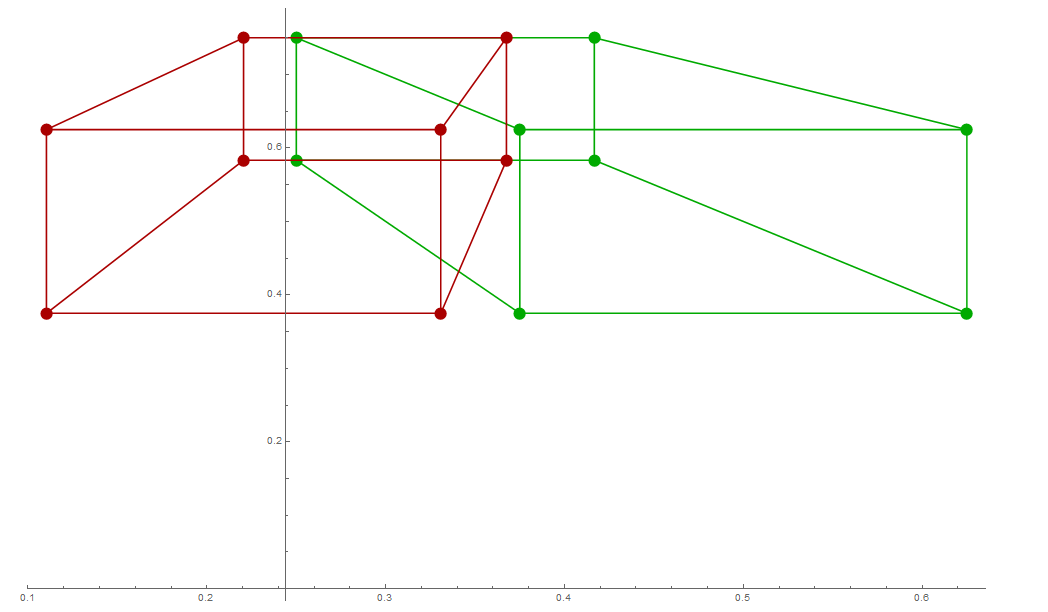
\includegraphics[width=1.\linewidth]{images/Rectification_HsHrHp_same_Solutions.png}
	\captionof{figure}{Abbildung beider Bilder nach anwenden der Matrizen $H_s \cdot H_r \cdot H_p$ und $H_s' \cdot H_r' \cdot H_p'$. Die horizontale Verzerrung wurde reduziert.} 
\end{minipage}\\ \\

\begin{minipage}{\linewidth}
	\centering
	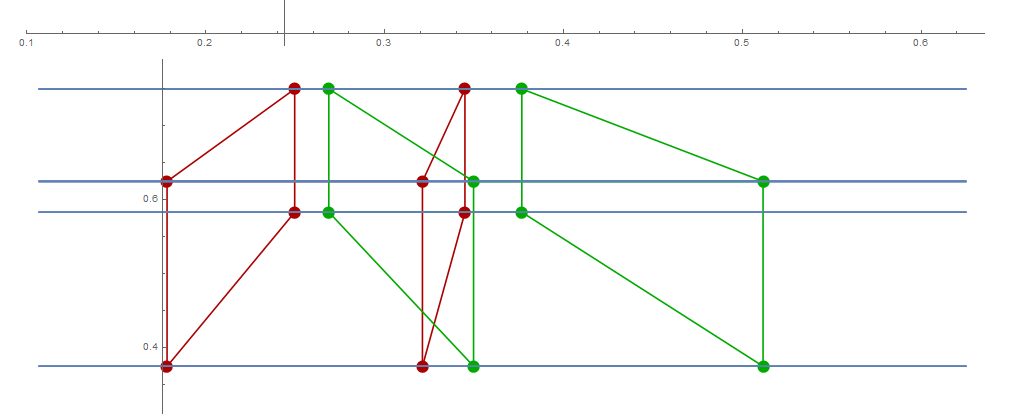
\includegraphics[width=1.\linewidth]{images/Rectification_four_same_Solutions.png}
	\captionof{figure}{In dieser Abbildung wurden die Epipolarlinien noch in den Grafikplot mit eingebaut} 
\end{minipage}\\ \\

%\begin{minipage}{\linewidth}
%	\centering
%	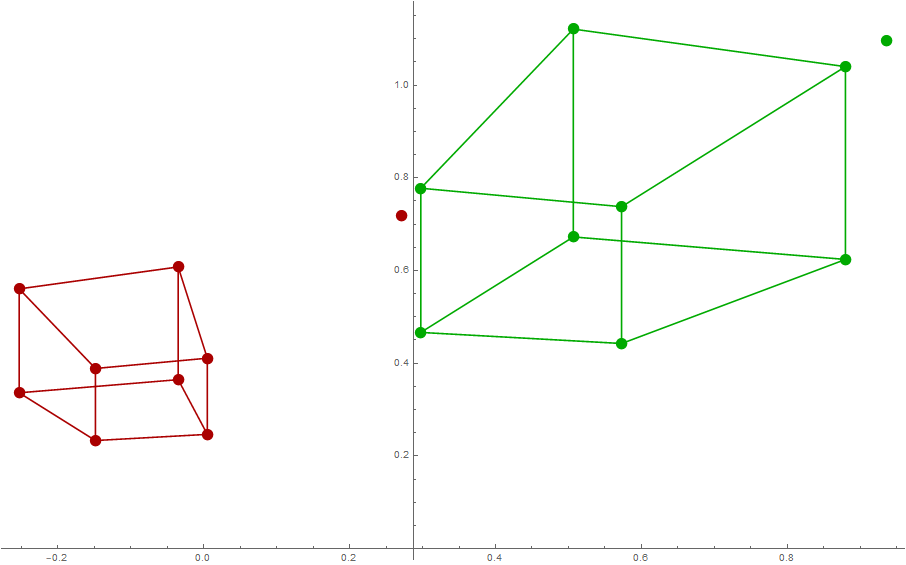
\includegraphics[width=1.\linewidth]{images/Rectification_one_different_Solutions.png}
%	\captionof{figure}{Aufnahmen zweier Kameras mit unterschiedlichen auflösungen, Kamera eins(Grün) besitzt für \ensuremath{\zeta} den Wert 1 und für Kamera zwei(rot) gilt jeweils \ensuremath{\zeta_x = 1.2} und \ensuremath{\zeta_y = 3.1}} 
%\end{minipage}\\ \\
%
%(Normalerweise in realbildern wird das bild bei unterschiedlicher Auflösung nicht verzerrt sondern nur "Vergrößert" oder zurecht "geschnitten". Dadruch dass beide Quader in einem Koordinatensystem verbaut wurden sieht das so aus)
%
%
%\begin{minipage}{\linewidth}
%	\centering
%	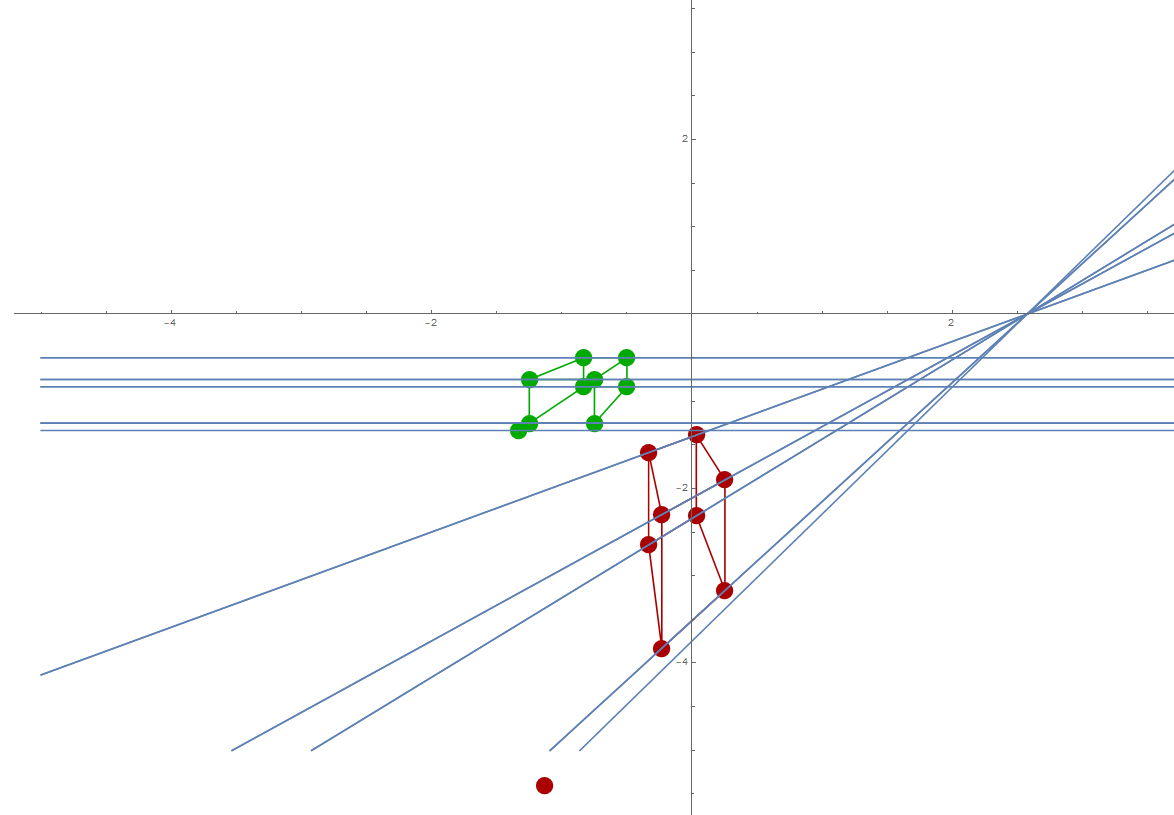
\includegraphics[width=1.\linewidth]{images/Rectification_two_different_Solutions.png}
%	\captionof{figure}{Epipole für Kamera eins und Kamera zwei vor der Rektifizierung } 
%\end{minipage}\\ \\
%
%
%\begin{minipage}{\linewidth}
%	\centering
%	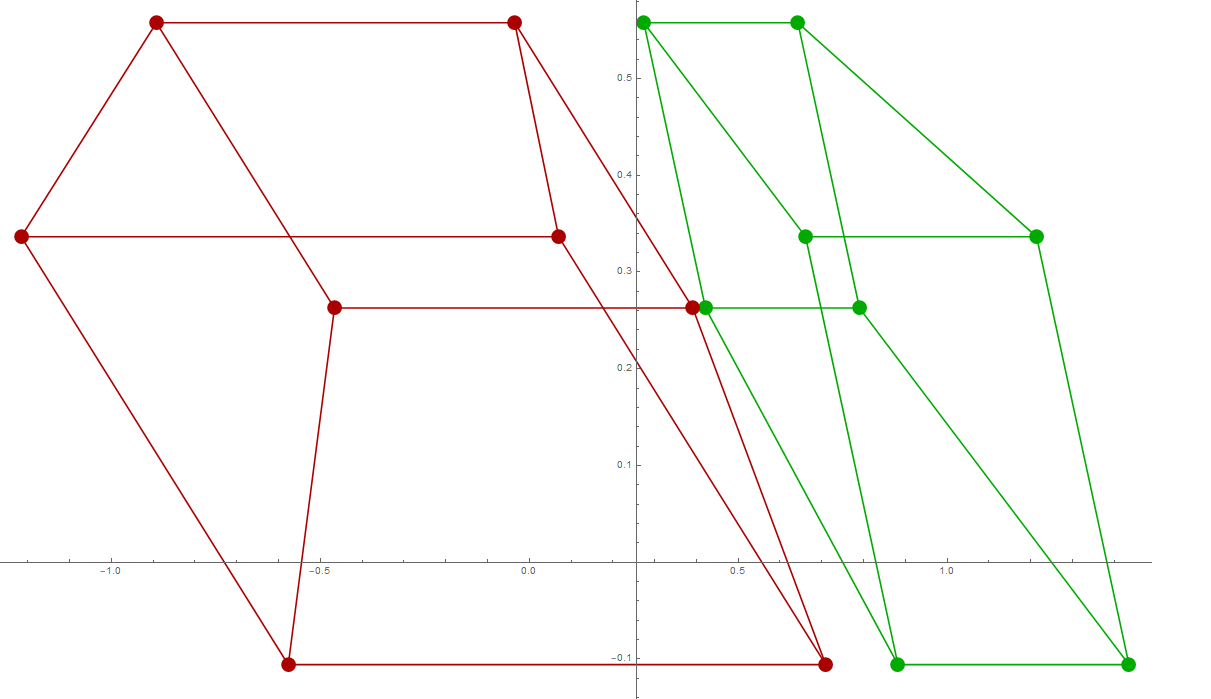
\includegraphics[width=1.\linewidth]{images/Rectification_three_different_Solutions.png}
%	\captionof{figure}{Nach dem die drei Homographien auf die Punkte angewandt sind die Eckpunkte des Quaders auf beiden Bilder auf den selben corresüondierenden Epipolarlinien} 
%\end{minipage}\\ \\
%
%
%\begin{minipage}{\linewidth}
%	\centering
%	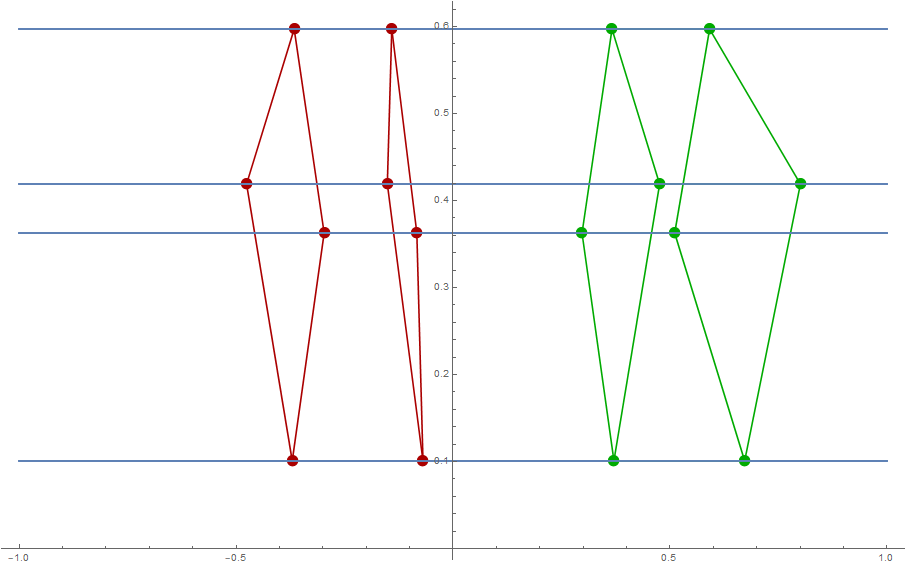
\includegraphics[width=1.\linewidth]{images/Rectification_four_different_Solutions.png}
%	\captionof{figure}{In dieser Abbildung wurden die Epipolarlinien noch in den Grafikplot mit eingebaut} 
%\end{minipage}\\ \\
